\documentclass[smallextended,natbib]{svjour3}       % onecolumn (second format)
\usepackage{graphicx}
\usepackage{newtxtext}
\usepackage{url}
\usepackage{lineno}

\renewcommand{\tablename}{Tab.}

\linenumbers

\begin{document}
	
%opening
\title{Pikunda-Munda and Batalimo-Maluba}
\subtitle{Archaeological Investigations of the Iron Age Settlement History of the western and northern Congo Basin}
%\titlerunning{Short form of title}        % if too long for running head

\author{}
%\author{Dirk Seidensticker}

%\institute{Dirk Seidensticker \at
%	Ghent University \\
%	Department of Archaeology \\
%	UFO, Sint-Pietersnieuwstraat 35 \\
%	B-9000 Ghent \\
%	\email{dirk.seidensticker@ugent.be}
%}

\date{Received: date / Accepted: date}
% The correct dates will be entered by the editor

\maketitle

\begin{abstract}
The spread of pottery-producing communities into the Congo rainforest is commonly linked to demic diffusion, driven by the so-called ‘Bantu Expansion’. It is considered the primary linguistic, cultural, and demographic process in Holocene sub-Saharan Africa. A key region in reconstructions of this process is the western Congo Basin. This paper presents, for the first time, a coherent picture of the archaeological settlement history in the western and northern Congo Basin, uncovered by fieldwork of the late 1980s along the rivers Ngoko, Sangha, Likwala-aux-Herbes, Ubangi, and Lua. Archaeological research of the \textit{River Reconnaissance Project}, directed by Manfred K. H. Eggert from 1977 to 1987, produced a pottery sequence for the Congo Basin. Archaeological features and findings uncovered during the project’s field campaigns in the northern and western Congo Basin have only recently been studied in detail. The present analysis provides the only reliable source for the a reconstruction of the cultural dynamics within the region due to lack of subsequent archaeological fieldwork. Archaeological data and the sequence of pottery styles within the western Congo Basin, along the Sangha river, cannot support the claim that this region, due to a climate-induced extension of savannas, played a unique role as a ‘corridor’ within the expansion of putatively ‘Bantu’ speaking groups during the latter half of the 1st millennium BCE.

\noindent\textbf{Résumé} La propagation des communautés productrices de poterie dans la forêt tropicale du Congo est généralement liée à une diffusion démique, entraînée par ce qu’on appelle "l’expansion Bantoue". Il est considéré comme le principal processus linguistique, culturel et démographique de l’Afrique subsaharienne de l’Holocène. Une région clé dans les reconstructions de ce processus est l’ouest du bassin du Congo. Cet article présente, pour la première fois, une image cohérente de l'histoire des peuplements archéologiques dans l'ouest et le nord du bassin du Congo, découverte par des travaux de terrain menés à la fin des années 1980 le long des rivières Ngoko, Sangha, Likwala-aux-Herbes, Oubangi et Lua. Les recherches archéologiques du \textit{River Reconnaissance Project}, dirigées par Manfred K. H. Eggert de 1977 à 1987, ont produit une séquence de poterie pour le bassin du Congo. Les caractéristiques archéologiques et les découvertes découvertes lors des campagnes de terrain du projet dans le nord et l’ouest du bassin du Congo n’ont été étudiées en détail que récemment. La présente analyse constitue la seule source fiable pour la reconstruction de la dynamique culturelle au sein de la région en raison du manque de travaux archéologiques ultérieurs sur le terrain. Les données archéologiques et la séquence des styles de poterie dans l'ouest du bassin du Congo, le long de la rivière Sangha, ne peuvent pas étayer l'affirmation selon laquelle cette région, en raison d'une extension des savanes induite par le climat, a joué un rôle unique de "couloir" dans l'expansion du pays. groupes de langue putativement "bantou" au cours de la seconde moitié du 1er millénaire avant notre ère.

\keywords{Congo Basin \and Pottery \and Iron Age \and Settlement History}
\end{abstract}

\section*{Introduction}\label{intro}

The archaeological sequence in the Inner Congo Basin or \textit{Cuvette central} has been studied in detail \citep{Wotzka.1995}, while finds from the adjacent western and northern fringes of the Congo Basin were analyzed only recently \citep{Seidensticker.2021e}. This region is critical as prevailing models of the spread of sedentary lifestyle in sub-Saharan Africa, regularly derived from linguistic reconstructions of modern languages, propose it as the route for substantial migrations \citep{Bostoen.2018,Bostoen.2020}. Relying on phylogenetic modeling and coupling their results with evolutionary genetic research, historical linguists favor rapid expansion, driven by demic diffusion, into and through the equatorial rainforests \citep{Currie.2013,Bostoen.2015,Grollemund.2015,Koile.2022,Grollemund.2023}. Regularly, these findings are coupled with an intensification of archaeological remains yielding ceramics in the second half of the 1st millennium BCE \citep{deSaulieu.2021a,Seidensticker.2021}.

While the key objective of the research summarized here, was to reconstruct the settlement history of the northern and western Congo Basin, by establishing a chrono-typological framework of pottery development \citep{Seidensticker.2021e}, this paper addresses three additional research questions: it gives a critical review of the "Sangha River Interval" (SRI) Hypothesis including the archaeological ground-truths, i.e. the missing signature of hypothesized migrations along the Sangha river valley during the 1st millennium BCE \citep{Currie.2013,Bostoen.2015,Grollemund.2015,Koile.2022,Grollemund.2023}. Furthermore, this paper addresses the decline in archaeological finds between the end of the Early Iron Age in the 5th to 6th century CE and the onset of the Late Iron Age in the 10th century CE, specifically a so far overlooked potential recess in human activity in the Congo Basin. At last, this study examines regional differences in pottery finds along the Ubangi river, hinting at a prolonged 'fuzzy border'.

\subsection*{History of Research}

Among the first archaeological finds from the northern Congo Basin are partially polished lithic artifacts, found during colonial times between Libenge, Dongo and Gemena \citep{Bequaert.1937,Bequaert.1938a,Bequaert.1940a,Bequaert.1946}. A first excavation was conducted at Batalimo on the Lobaye river, a tributary of the Ubangi river, by Roger \citet{DeBayleDesHermens.1969,DeBayleDesHermens.1971,deBayledesHermens.1975}. The site was first discovered in 1966 during construction works, and a 2~\texttimes~3~m big trench was excavated in 1968. The site was revisited in 1981 by Pierre Vidal and most notably between 1987 and 1990 by Lassina \citet{Kote.1992}. More recent excavations directed by Alfred Jean-Paul \citet{Ndanga.2010} focused on re-evaluating the cultural layer discovered by \citet{deBayledesHermens.1975}, and the debated co-occurrence of partially polished lithic artifacts and ceramics \citep[137]{Eggert.1987c}. In the early 1970s, Francis \citet{vanNoten.1978} conducted fieldwork in the Ubangi region. Two notable sites were excavated, the rock-shelter of Hau, to the west of Gemena, and Motenge-Boma on the middle Ubangi river (Fig.~\ref{fig:map}). The excavation at Hau revealed three distinct layers, each characterized by a specific inventory. The lowest layer contained lithic artifacts in Levallois technique and was thus dated into the Middle Stone Age \citep[27,30]{vanNoten.1982d}. Above that was a layer with microliths, associated with the Late Stone Age, while the uppermost layer was characterized by potentially Iron Age pottery \citep[31]{Bahuchet.1992}. Unfortunately, three charcoal samples, one from each layer, were unsuccessfully radiocarbon dated, ending all studies of the material as the site was deemed disturbed \citep[27,30]{vanNoten.1982d}. Motenge-Boma, the second site excavated by \citet{vanNoten.1978} yielded a few remains of pottery, all showing carved roulette \citep[Fig.~40]{vanNoten.1982} and dating into the Late Iron age.

Between 1977 and 1987, extensive boat surveys along the tributaries of the Congo river were performed in the context of the \textit{River Reconnaissance Project}, directed by Manfred K. H. \citet{Eggert.1983,Eggert.1984,Eggert.1993,Eggert.1996}. A detailed analysis of this project’s discoveries in the Inner Congo Basin, south of the Congo river, has been published by Hans-Peter \citet{Wotzka.1993}. Wotzka’s reconstruction of the settlement history of the \textit{Cuvette central} relies on a sequence of 35 pottery styles that span the last two-and-a-half millennia and pertain to six stylistic traditions. Four more local stylistic traditions, named after their main region of distribution "Luilaka", "Tshuapa", "Busira", and "Maringa" show interconnections that were indicative of them sharing a common ancestry within the "West tradition" \citep[219--225 Fig.~4]{Wotzka.1995}. \citet{Wotzka.1995} condensed this evolutionary development into the "Equator-Co style tradition", applying the concept similar to \citet{Rouse.1957}, \citet{Huffman.1970}, \citet{Schmidt.1975}, \citet{Vogel.1978}, and \citet{Hall.1983}. The initial phase of pottery in the Congo Basin dates from 400 to 200 BCE and is represented by the Imbonga style \citep[59--68]{Wotzka.1995}. The expansion continued into the 16th century CE, and the first settlers did not penetrate the entire region at once. Instead, the settling of the Inner Congo Basin occurred in multiple successive waves of upriver expansions \citep[226--241]{Wotzka.1995}. \citet[290]{Wotzka.1995} concludes that "the explored parts of the Inner Congo Basin constitute a remarkably self-containing ceramic sphere in the course of the last 2 400 years" and that "all [encountered] pottery styles could be traced back to the Imbonga group".

Aiming at uncovering the northern extent of the Imbonga style, fieldwork of the \textit{River Reconnaissance Project} was extended along the Ubangi river and its tributary, the Lua river, in 1985 \citep{Eggert.1987c}. The survey traversed the equatorial rainforest up to the tropical savanna (Fig.~\ref{fig:map}). The roughly 850~km long exploration of the Ubangi yielded 44 sites, of which only the site of Motenge-Boma had been published prior \citep[75]{vanNoten.1978,vanNoten.1982a}. Four additional sites were discovered along an approximately 100~km long stretch of the lower Lua river, most notably Maluba, where multiple pit features were excavated. The only other site with an equally distinct record like that uncovered at Maluba is Batalimo on the Lobaye river \citep{DeBayleDesHermens.1969,DeBayleDesHermens.1971,deBayledesHermens.1975}.

After the surveys along the Ubangi and Lua, which did not yield pottery associated with the earliest styles from the Inner Congo Basin, the campaign of 1987 focused on the western parts of the Congo Basin \citep[Fig.~\ref{fig:map};][]{Eggert.1992}. The nearly 600~km long survey of the Sangha river, from its mouth at Mossaka – around 220~km south of Mbandaka – up to Bomasa at the border triangle of the Republic of the Congo, Cameroon, and the Central African Republic, yielded 38 new sites. A survey along a roughly 80~km long stretch of the Ngoko river, which joins the Sangha north of Ouesso, added another eight sites. The last survey, the \textit{River Reconnaissance Project} conducted in 1987, covered the Likwala-aux-Herbes river, which runs in-between the Ubangi and Sangha and is characterised by a very distinct ecology \citep{Philippon.2019}. The Likwala-aux-Herbes, not to be confused with the Likwala-Mossaka running further west, is characterised by a swampy bush- and grassland. Higher vegetation only appears multiple kilometres away from the river. Thus, a vast floodplain can be found at each river bank, unlike along the Sangha river, where the rainforest vegetation reaches directly to the river bank. The 530 km long survey yielded another 23 sites. The entire region surveyed was archaeological \textit{terra incognita} before 1987. The project’s discoveries, including preliminary results from the western and northern Congo Basin, were outlined in a well-known paper concerning the archaeology of the equatorial rainforest \citep{Eggert.1993}. The survey and excavation finds were partially summarized \citep{Seidensticker.2016b} until the detailed analysis was published recently \citep{Seidensticker.2021e}. 

Fieldwork in the region re-commenced during the past decade. Contrasting earlier endeavours is the prevalent integration of paleo-ecological research. Focal points of research have been the Ngoto forest reserve in the south-western parts of the Central Africa Republic \citep{Kiahtipes.2011,Lupo.2015,Kiahtipes.2016,Lupo.2021}, the northern parts of the Republic of the Congo \citep{Gillet.2013,MorinRivat.2014,Morin-Rivat.2017a}, the north-eastern parts of the Congo Basin \citep{Cornelissen.2013,LivingstoneSmith.2011,LivingstoneSmith.2017}, as well as the Inner Congo Basin \citep{Neumann.2022}.

\subsection*{Material culture and language}

A defining paradigm when working with pottery finds from Central Africa concerns the imposed link between this category of material culture and languages. The prevailing model of the spread of sedentary lifestyle proposes a 'migration' of Bantu-speech communities through the rainforest, often identified by the presence of pottery finds \citep{Currie.2013,Bostoen.2015,Grollemund.2015,Koile.2022,Grollemund.2023}. At the core of an intense academic debate surrounding the term 'Bantu' \citep[cf.][]{Oliver.1966,Vansina.1979,Vansina.1980,Robertson.2000,Eggert.2005,Eggert.2016a} lies a profound conceptual trend in which a "purely technical [term] without any non-linguistic connotations [that] was transformed into a designation referring indiscriminately to language, culture, society, and race" \citep[302]{Eggert.2005}. Research of the modern, about 300-600 languages spoken in sub-Saharan Africa summed up within the Bantu language family \citep{Nurse.2003,Bostoen.2018}, resulted in two main models aimed at explaining their dispersion: an 'early split' of languages with predicted migrations on the northern fringes of the rainforest and a 'late split' model with migrations through the rainforest and subsequent diversification \citep{Bostoen.2018,Bostoen.2020}. \citet{Pakendorf.2011} claim that evolutionary genetic research on modern communities points towards demic diffusion as the driving force behind the expansion of Bantu languages in favor of the distribution of languages and technologies \citep{Bostoen.2022}. While migrations are incorporated into such models for the initial spread of speech-communities, their more recent dynamic histories \citep[cf.][83]{Vennetier.1963} are equally omitted as setbacks in human activity \citep{Oslisly.1998,Oslisly.2013b,Saulieu.2017,deSaulieu.2021a,Seidensticker.2021}. \citet[1]{Lipson.2022} point out that "the structure of ancient populations cannot be robustly reconstructed based solely on genetic data from present-day people" due to disruptions by "demographic transformations", including "colonialism, imperialism, enslavement, and modern sociopolitical reorganization".

An unfortunate but common practice in order to 'date' nodes in linguistic reconstructions of modern Bantu languages is 'calibrating' them using archaeological data: for example, \citet[SI p.~2]{Grollemund.2015} equates an initial off-branching in the Cameroon-Nigeria homeland with the archaeological inventories of the lower horizon of the Gray Ash layer from the site of Shum Laka, representing the second phase of the "Stone to Metal Age" (SMA) or "Ceramic Late Stone Age" and dating into the 3rd to 2nd millennium BCE \citep[226--231,243]{Lavachery.2001}. During that phase the microlithic quartz industry, dominating the late Pleistocene deposits \citep[172 Fig.~4]{Cornelissen.2003,Cornelissen.2017}, is slowly declining, while a macrolithic flake and blade industry on basalt, which occurs in smaller numbers in older deposits as well, becomes more prevailing \citep[169 Fig.~1]{Cornelissen.2003,Cornelissen.2017}. Pottery, while already present in the older deposits of the upper horizon of the Ochre Ash layer and dating into the 5th to 4th millennium BCE \citep[224-225 Fig.~4.2--3]{Lavachery.2001}, is now more prominent and decorated with grooves and impressions, including rocker zig-zag \citep[231--232 Fig.~8]{Lavachery.2001}. It must be stressed that Shum Laka represents the only site in the wider region of the putative homeland of the Bantu languages, in the border area of Nigeria and Cameroon, that has been studied in detail. Thus the deciding factors of \citet{Grollemund.2015} for 'selecting' the specific deposits at Shum Laka as an archaeological 'calibration point' for their phylogentic language tree is neither quantitative nor qualitative. And while \citet[SI p.~2]{Grollemund.2015} allege that "small immigrant communities from further north" introduced pottery and Benue-Congo languages, more recent genetic analyses from four burials at Shum Laka showed that the genetic profiles of the occupants of the site "are very different from those of most speakers of Niger–Congo languages today, which implies that these individuals are not representative of the primary source population(s) that were ancestral to present-day Bantu-speakers" \citep[5]{Lipson.2020}. 

\citet[SI p.~2]{Grollemund.2015} date the subsequent node of Bantu languages in the younger half of the 2nd millennium BCE based on the earliest occurrence of markers for 'sedentism' at Obobogo in southern-central Cameroon \citep{deMaret.1982,deMaret.1983,deMaret.1992}. It must be noted that final analyses from the site of Obobogo are still pending. \citet{Claes.1985} provided some initial results, but not a consecutive analysis of all available data. \citet[SI p.~2]{Grollemund.2015} associate the third mayor branching-off point with the emergence for Urewe ceramics in the Great Lakes region of East Africa. All these choices together perpetuated the trope that early Bantu-speakers can be equated with the earliest pottery production in a given region \citep[355,362,364]{Bostoen.2015}. This generalization further suffers from disregarding the (dis-)continuities of a single facet of material culture in a given region and their relations to any historically identifiable human society. In a nutshell, the procedure of adopting opportune archaeological results for underpinning linguistic reconstructions by \citet{Grollemund.2015} and \citet{Bostoen.2015}, which was subsequently adopted by \citet[SI]{Koile.2022} without any critical review, represents another facet of a long-standing tradition in circular reasoning \citep{Ehret.1973,Phillipson.1976,Phillipson.1976b,Phillipson.1977a,Heine.1977} that has been reviewed by \citet[82]{Eggert.2005,Eggert.2016a}. Such approaches induce 'procedural puzzles' and fail at linking linguistics with "the authentic material evidence of archaeology" \citep[88]{Eggert.2016a}. In consequence it can only be reiterated that "non-written languages do not leave material traces" \citep[85]{Eggert.2016a}.

\begin{figure*}[!tb]
	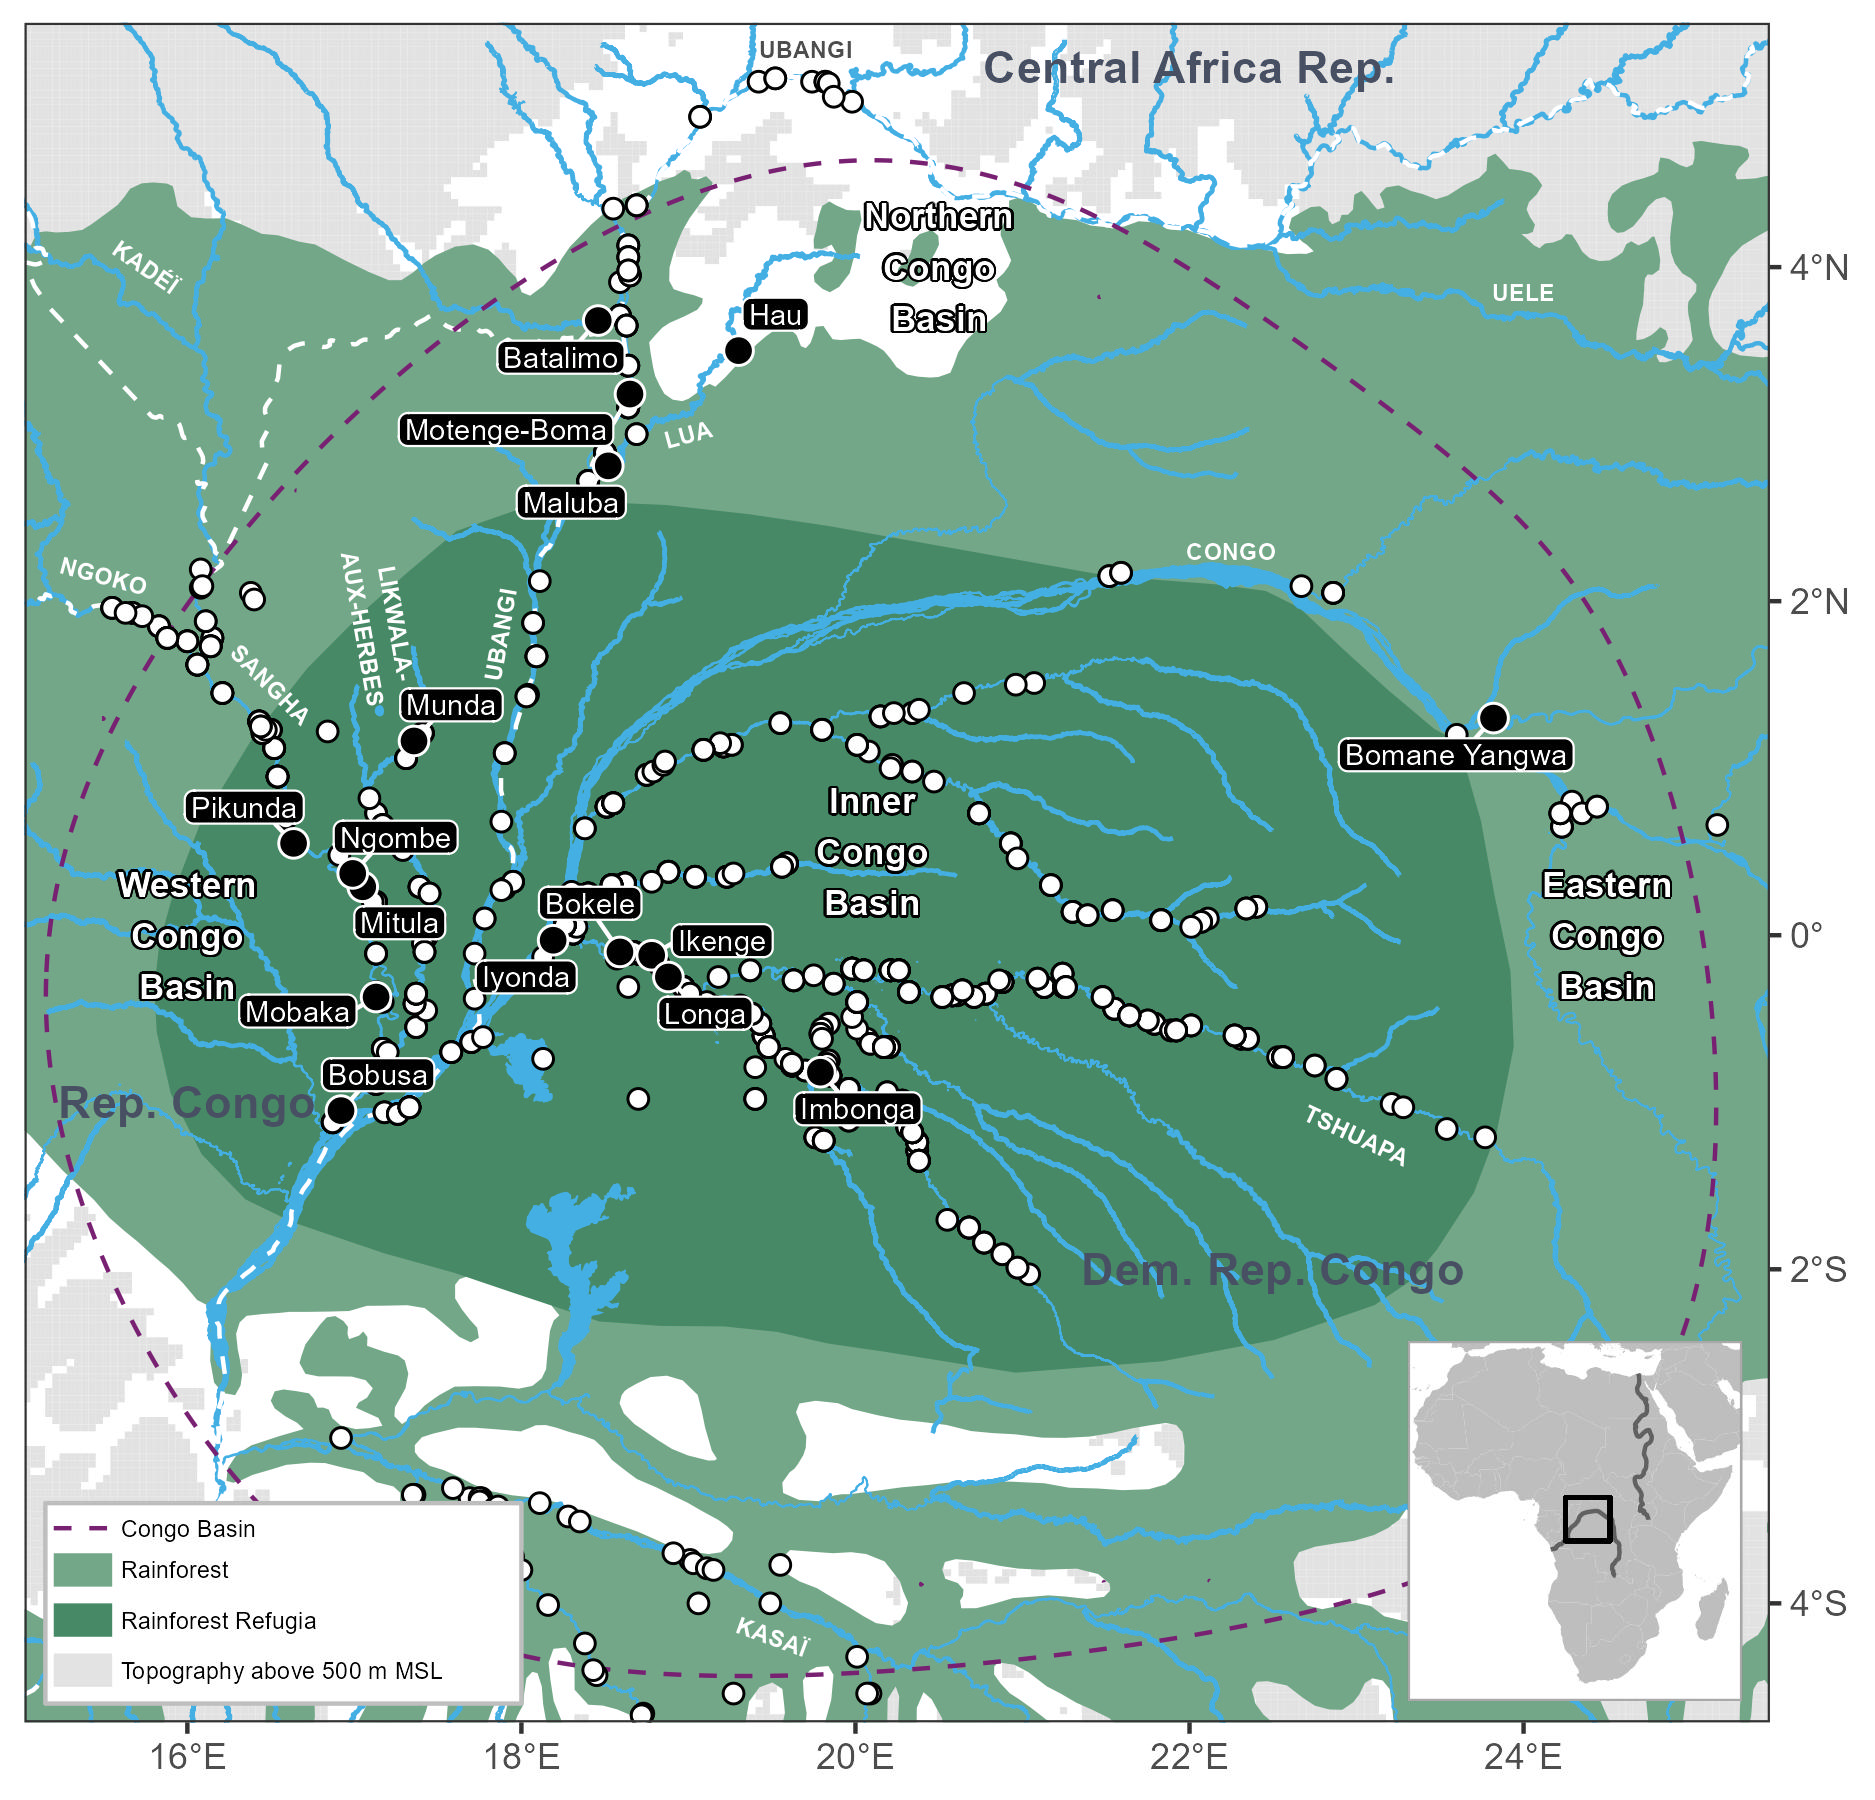
\includegraphics[width=\textwidth]{fig_map.pdf}
	\caption{Map of the Congo Basin. White dots are known sites with pottery finds (dark dots representing sites mentioned in the text). Green shading shows the modern extent of the equatorial rainforest \citep{White.1983}. Dark green shading represents the putative extent (refugia) of the rainforest during the 1st millennium BCE rainforest crisis \citep{Bremond.2017,Maley.2017}. The purple dotted line shows the extent of the Congo Basin \citep[11]{Runge.2001}. Grey shading shows topography above 500 m ASL.}
	\label{fig:map}
\end{figure*}

\subsection*{Landscape and Geography}

The study area is a north-south transect through the rainforest, as most surveyed rivers run north to south. It covers the tropical savanna climate ('Aw'-climate according to the Köppen-Geiger systematic) in the north, followed by the tropical monsoon climate ('Am'), while the bulk of sites is located in tropical rainforest climate \citep['Af';][]{Peel.2007}. At the heart of the study area lies the Congo Basin, which is dominated by the Congo river and its many tributaries. The catchment area of the Congo river covers the entire area of the Democratic Republic of the Congo (DRC) as well as large parts of the Republic of the Congo, south-eastern Cameroon, the southern Central African Republic and adjacent areas further east, south-east and south of the DRC \citep[60 Fig. 1]{Eggert.2017}. The Congo Basin is generally limited to a topography below 450 m ASL \citep[11]{Runge.2001} and characterized by quaternary geological deposits \citep{Persits.1997}.

For this review of the settlement processes, the study area is represented best when subdivided into the “western Congo Basin” (rivers Ngoko, Sangha and Likwala-aux-Herbes) and the “northern Congo Basin” (region of the Ubangi and Lua river) (Fig.~\ref{fig:map}).

\section*{Materials and Methods}\label{materials}

The research is based on inventories of 122 sites along the rivers Ubangi, Lua, Sangha, Ngoko, and Likwala-aux-Herbes (Fig.~\ref{fig:map}). The study area covers an area of about 500\,$\times$\,700 km. In total, the studied collection is comprised of around 10.500 individual objects, including roughly 4.200 vessel units and a similar amount of highly fragmented ceramic sherds \citep[23--43]{Seidensticker.2021e}. At five sites, 14 features were excavated. Most of the excavated features were pits. Additional pit features were sampled at four sites. Only about a third of the studied ceramics was discovered during excavations or deliberate sampling of clearly identifiable features.

Morphologically and ornamentally similar vessel units are summarized as pottery styles, following the established conceptualizations of \citet[52--57]{Wotzka.1995}. The styles describe a specific and recognizable way ceramics are produced and decorated. Throughout the text, the term 'group' is used synonymous for 'style'. Additionally, early investigations into clay sourcing, conceptualized as macroscopic pottery fabrics \citep[60--69]{Seidensticker.2021e}, were included in the morphological description of ceramic styles.

The study’s main objective was to develop a spatio-temporal reference framework for the area based on pottery groups derived from the ceramics' technological, morphological, and ornamental characteristics. Twenty-four new ceramic style were described for the northern and western Congo Basin combined. Furthermore, five styles found mainly within the Inner Congo Basin and described by \citet{Wotzka.1995} could be identified.

Established concepts were adopted (\citeauthor{Eggert.1983} \citeyear{Eggert.1983}, 295; \citeyear{Eggert.1984}, 250, 257; \citeyear{Eggert.1988}, 28--31; \citeauthor{Wotzka.1995} \citeyear{Wotzka.1995}, 217--225) to describe the change and development of pottery in the study area. A sequence of subsequent pottery styles that share clear indications that one was derived of the other are regarded as ‘pottery traditions’ or ‘style traditions’ \citep{Rouse.1957,Willey.1945}, while contemporaneous sets of closely related pottery styles are summarized as ‘style horizons’ \citep[108--111]{Kroeber.1944}.

All data and computer code produced are available here: \url{https://github.com/dirkseidensticker/PikundaMunda_BatalimoMaluba_AAR}

\begin{table*}[p]
	\centering
	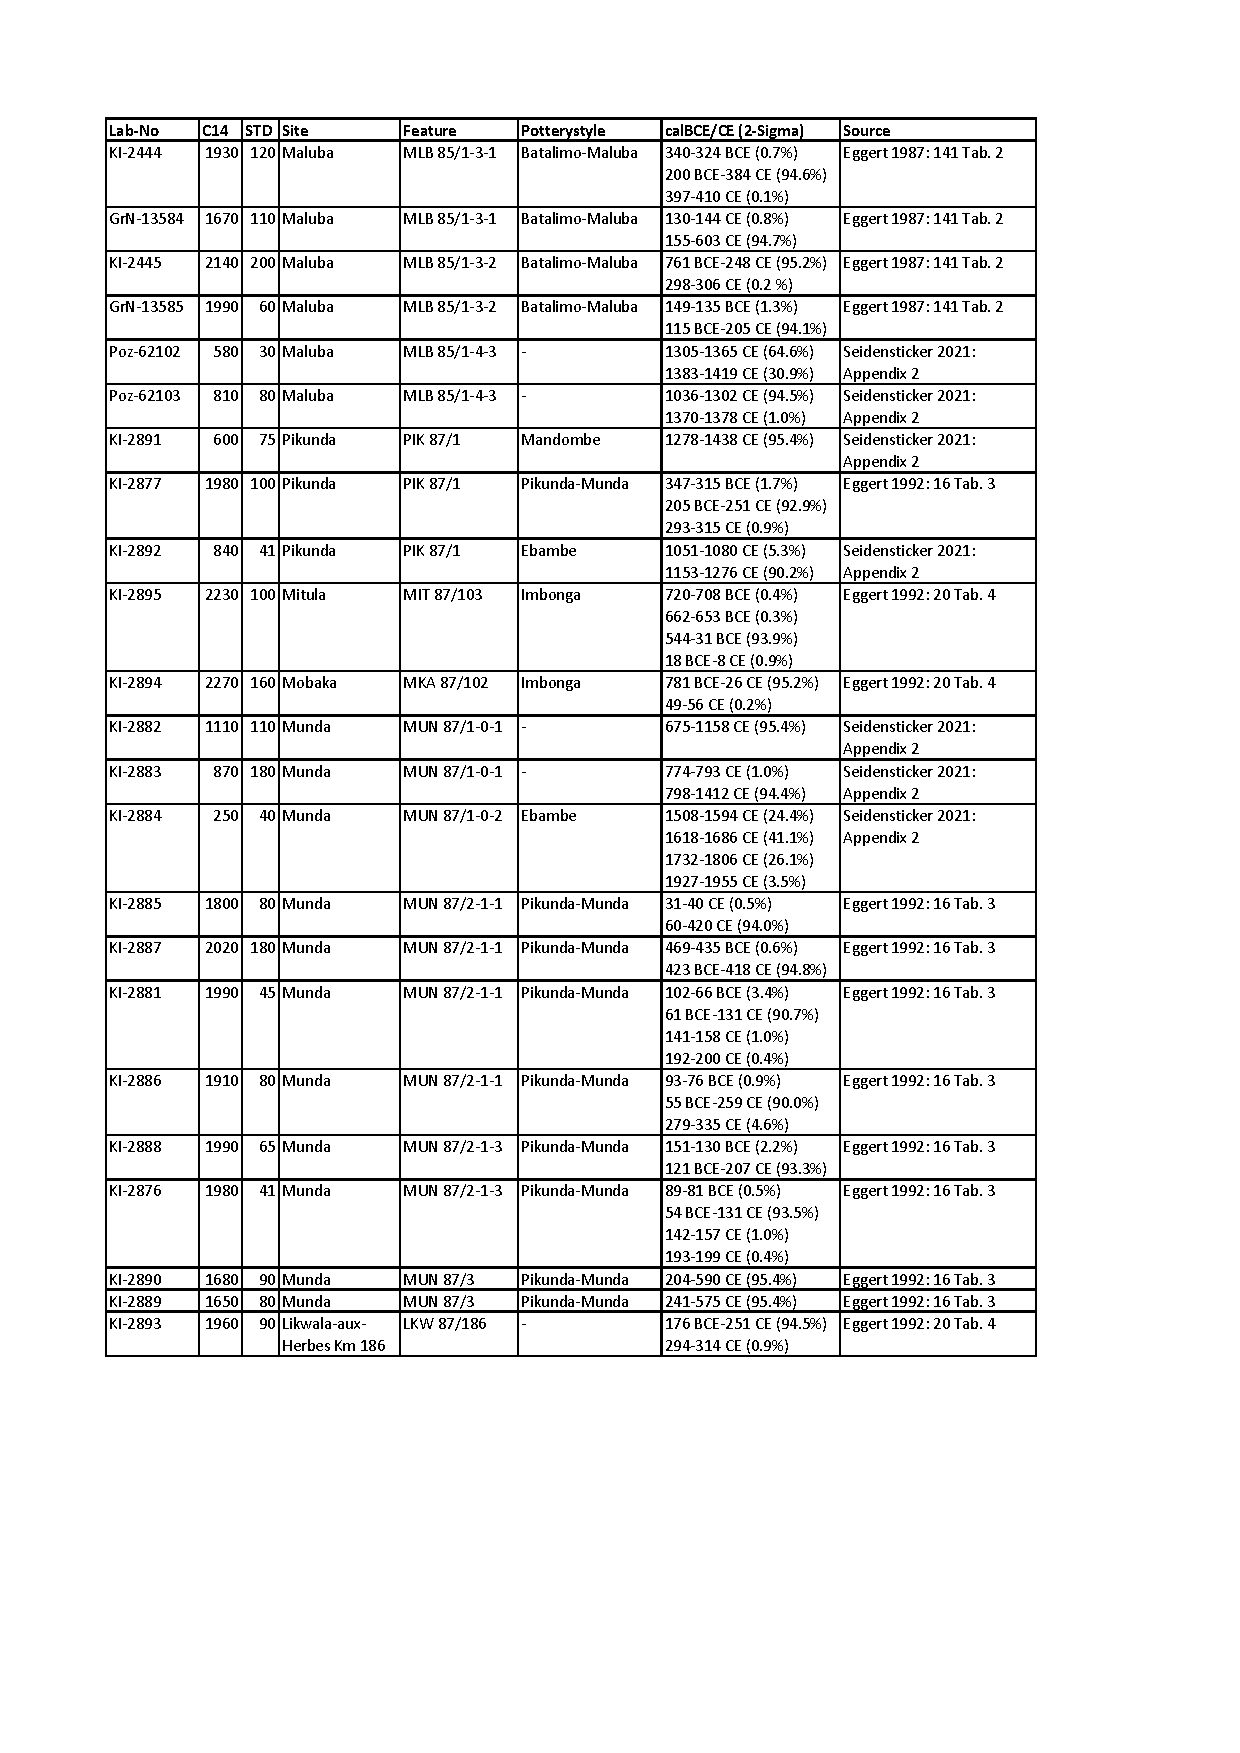
\includegraphics[width=.9\textwidth]{Tab_Old14C.pdf}
	\caption{Calibrated ages \citep{Reimer.2020} of previously published radiocarbon dates from the fieldwork of the \textit{River Reconnaissance Project} in the western and northern Congo Basin \citep[Appendix 2]{Seidensticker.2021e}.}
	\label{tab:14Cold}	
\end{table*}

\begin{table*}[p]
	\centering
	
\includegraphics[width=.9\textwidth]{Tab_New14C.pdf}
	\caption{Calibrated ages \citep{Reimer.2020} of newly obtained AMS dates of foodcrusts from the interior of ceramic vessels and stable isotope values. Legacy radiocarbon dates can be found in Tab.~\ref{tab:14Cold}, the online aDRAC repository \citep{Seidensticker.2021f} and as a supplementary data table (Data S1).}
	\label{tab:14Cnew}	
\end{table*}

\subsection*{Radiocarbon Dating}

In total, 21 conventional radiocarbon samples were dated in the 1980s (Tab.~\ref{tab:14Cold}). All dates were obtained from charcoals found within the respective feature. Two additional samples from bone material were AMS dated in 2014 \citep[355--356 Appendix 2]{Seidensticker.2021e}. All dates are available via the aDRAC online repository \citep[\url{https://github.com/dirkseidensticker/aDRAC};][]{Seidensticker.2021f} and thus not listed individually here. Four samples obtained off food crusts from the interior of ceramics were AMS dated, providing for the first time direct and precise dates associated with the usage of the pottery (Tab.~\ref{tab:14Cnew}). Stable carbon and nitrogen isotopes were also measured to compensate for fresh-water reservoir effects.

\subsection*{Bayesian Phase Modeling}

The previously determined chronological ranges of the pottery groups \citep{Seidensticker.2021e, Seidensticker.2021} were further examined using Bayesian phase modeling. While \citet{Crema.2020a} relied on the OxCal software to run their model, an implementation that is available via the nimbleCarbon R-package was used \citep{Crema.2021a,Crema.2021b}. The code used to define the model was derived of the vignette provided with the nimbleCarbon software. A simple Bayesian chronological model was fitted to all radiocarbon dates of a given pottery style that showed sufficient archaeological contextualization and have not been discarded as potential lab errors in prior studies \citep[9]{Seidensticker.2021} and posterior probabilities for its onset and end were recovered (Fig.~S1). To compare these with the conventional estimations provided in earlier studies \citep[\url{https://github.com/dirkseidensticker/aSCAC};][Data S2]{Seidensticker.2021}, the median age value of the posterior distribution was extracted (Tab.~S1).

\section*{Results}

\subsection*{Early Iron Age (200 BCE – 500 CE) in the Western Congo Basin}

\subsubsection*{Imbonga style}

Remnants of the oldest ceramics in the western Congo Basin are found at two sites along the lower Sangha river, at Mitula and Mobaka \citep[Fig.~\ref{fig:map};][169--172, 306--307]{Seidensticker.2021e}. At both villages, fragments of diagnostic vessels were found partially embedded in the soil, indicating eroded remains of pit features. During the pottery's extraction, charcoal was found and subsequently radiocarbon dated. Charcoal from inside the vessel at Mobaka dates to the 8th to 1st centuries BCE (KI-2894; Tab.~\ref{tab:14Cold}), while the sample from underneath the vessel at Mitula dates to the 6th to 1st centuries BCE (KI-2895; Tab.~\ref{tab:14Cold}; Fig.~\ref{fig:chrono}). Both conventional radiocarbon dates show substantial standard errors and thus cover long timespans after calibration. These dates correspond to the age of the Imbonga style from the Inner Congo Basin, dated to the 4th to 1st centuries BCE and constituting the initial phase of settlement history in the Congo Basin \citep[Fig.~\ref{fig:chrono}; S1; Tab.~S1;][59--68]{Wotzka.1995}. The Imbonga style is characterized by vessels with flat bases that either show round bellies, pronounced shoulders, and profiled rims or are wide-mouthed bowls. Its decoration patterns comprise of rocker-stamping on the lower half, often combined with horizontal grooves and incised or plastic ornamentation on the vessels' shoulder regions \citep[196 Fig.~93.1--4]{Seidensticker.2021e}. The two mentioned vessels found on the lower Sangha river do not represent classic Imbonga characteristics but show striking similarities to vessels associated with the Imbonga style \citep[170 Fig.~84]{Seidensticker.2021e}: the vessel found at Mitula resembles another from Iyonda \citep[441 Pl.~7.7]{Wotzka.1995} while the vessel from Mobaka matches one found at Bokele \citep[453 Pl.~19.10]{Wotzka.1995}. These relatively isolated finds indicate an area of influence the Imbonga group had west of its previously known boundary.

\begin{figure*}[!tbp]
\centering
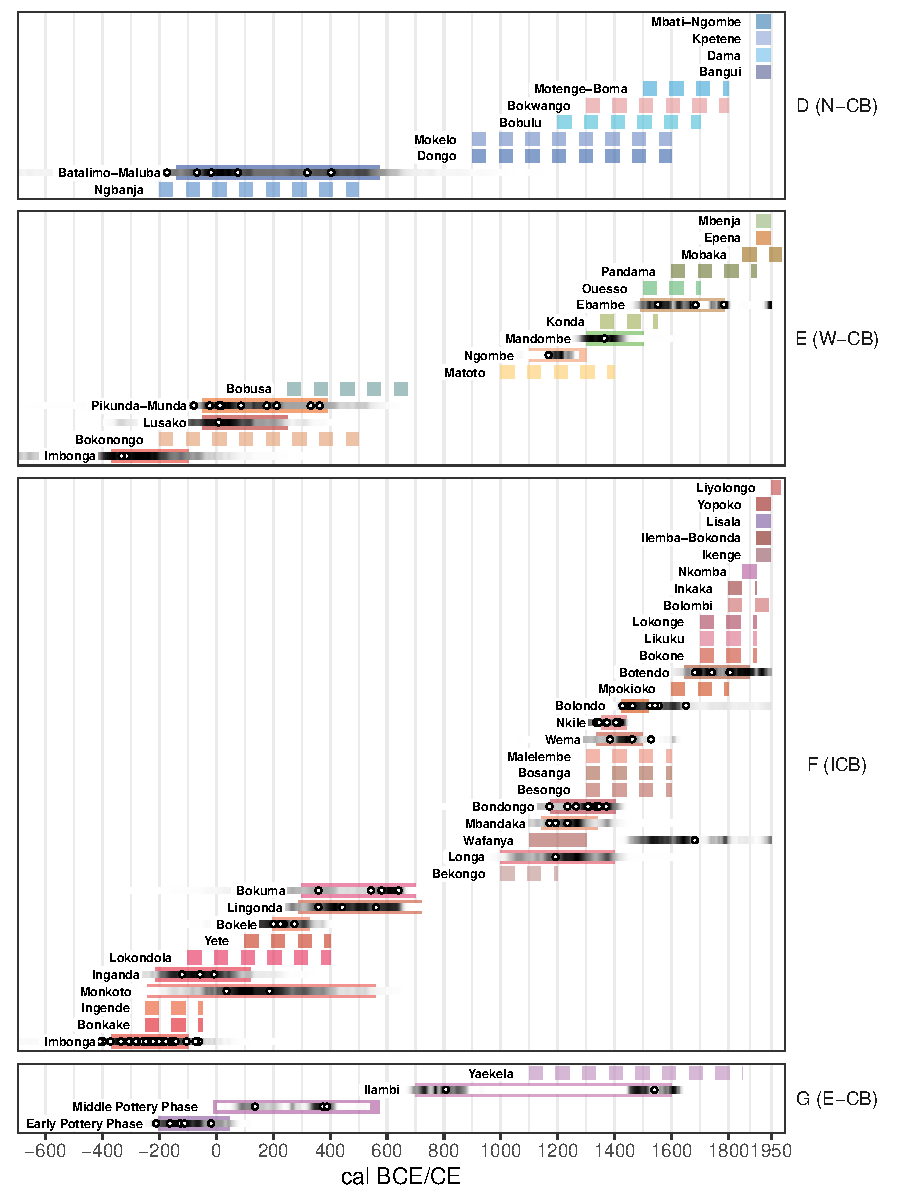
\includegraphics[width=\textwidth]{fig_chronology.pdf}
\caption{Temporal distribution of known pottery styles in the Congo Basin over the past 2600 years separated by regions \citep[Fig. 1; D) Northern Congo Basin, E) Western Congo Basin, F) Inner Congo Basin, G) North-Eastern Congo Basin]{Seidensticker.2021}. Circles represent the highest probability of calibrated calendar age of each pottery-linked 14C date. The intensity of grey-shading is proportional to the summed probability of the calendar-age windows of all pottery occurrences by type. Colored bars represent the phase duration of radiocarbon dated pottery styles. For groups with more than two associated radiocarbon dates, the median start and end dates of the phases were calculated using a Bayesian phase model (Fig.~S1; Tab.~S1). Dashed colored bars indicate estimated 100-year bins derived from stylistic resemblance \citep[Data S2]{Seidensticker.2021}.}
\label{fig:chrono}
\end{figure*}

\begin{figure*}[!tb]
	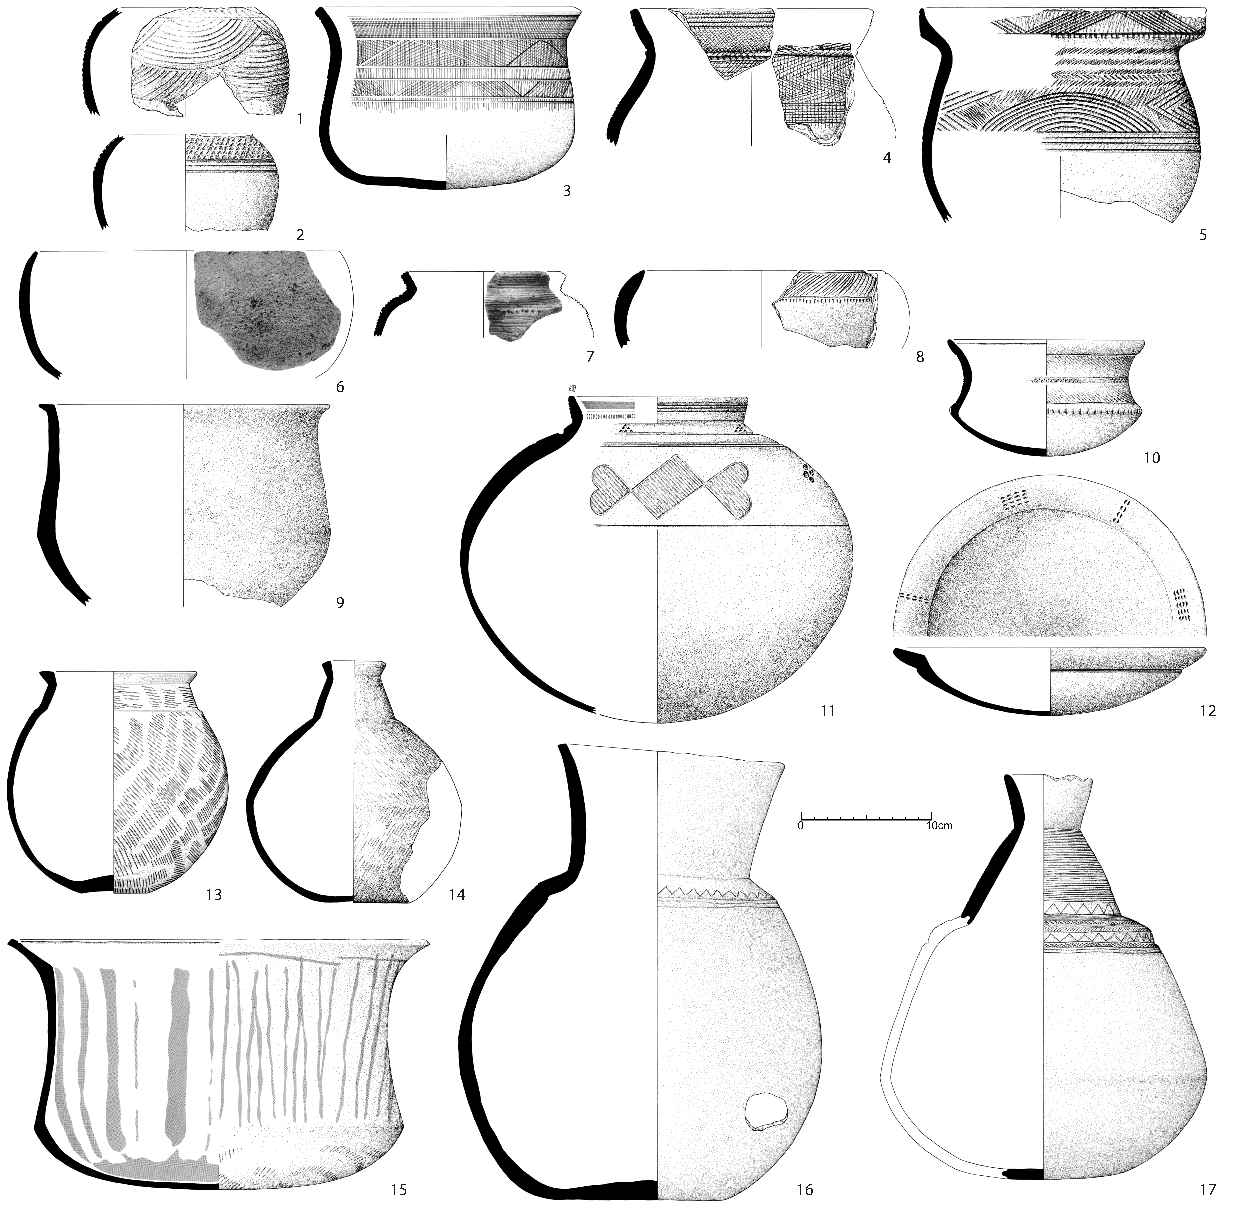
\includegraphics[width=\textwidth]{Sangha_Typen.pdf}
	\caption{Ceramic vessels from the western Congo Basin -- along the rivers Ngoko, Sangha and Likwala-aux-Herbes -- that are representative for the following pottery styles: 1--2) Imbonga; 3--4) Pikunda-Munda; 5) Bokonongo; 6--8) Bobusa; 9) Matoto; 10--12) Ngombe; 13--14) Ebambe; 15) Mobaka; 16--17) Epena \citep[114--144, 162--172]{Seidensticker.2021e}.}
	\label{fig:sangha}
\end{figure*}

\subsubsection*{Pikunda-Munda style}

The Pikunda-Munda group represents the earliest pottery style in the western parts of the Congo Basin \citep[114--120]{Seidensticker.2021e}. It shows substantial similarities to the contemporaneous groups in the Inner Congo Basin regarding pottery technology and decorations. However, concerning vessel shapes, there are considerable differences \citep[107 Ftn.~4]{Wotzka.1995}. The Pikunda-Munda style is represented best through the inventories of pit features excavated in 1987 at the two eponymous sites: Pikunda on the middle Sangha river and Munda on the upper Likwala-aux-Herbes river (Fig.~\ref{fig:map}). The excavation at Pikunda detected two features: one about 3.4~m deep pit dating from the 4th century BCE to the 3rd century CE (KI-2877; RICH-30864; Tab.~\ref{tab:14Cold}; \ref{tab:14Cnew}) that's been intersected by a considerably younger pit \citep[288--300]{Seidensticker.2021e}. The older pit contained two nearly complete vessels and around 160 sherds that can be attributed to the Pikunda-Munda style, as well as one rim sherd of the Lusako style known from the Inner Congo Basin (\citeauthor{Eggert.1992} \citeyear{Eggert.1992}, 18 Fig.~4.1; \citeauthor{Wotzka.1995} \citeyear{Wotzka.1995}, 104–-107). Four sherds show a considerably different fabric, shape, and decoration similar to that of the Ngbanja pottery known from the middle Ubangi river \citep[296 Tab.~34]{Seidensticker.2021e}. At Munda, two pits and a metallurgy-related feature yielded inventories of the Pikunda-Munda style \citep[321--339]{Seidensticker.2021e}. All features dated between the 1st century BCE and 4th century CE (Fig.~\ref{fig:chrono}; S1; Tab.~S1). The inventories from these pits are quite different compared to the one excavated at Pikunda, whose pottery is heavily fragmented. The pits at Munda contained complete vessels intentionally deposited either upside-down or lying on their side; a practice reminiscent of the depositions in pits in the Inner Congo Basin \citep{Wotzka.1993}. Overall nearly 550 vessel units are attributed to the Pikunda-Munda style, with two-thirds of the assemblage originating from the excavations mentioned above at the two eponymous sites.

Pikunda-Munda pottery was found along the Sangha river from its mouth into the Congo river in the south up to the village of Ikelemba, around 65~km south-east of Ouesso, and along the entire stretch of the Likwala-aux-Herbes river \citep[Fig.~\ref{fig:timeslices_1_eia}B--D;][119 Fig.~49]{Seidensticker.2021e}. A vessel from Ingonda Bosopela along the lower Lulonga river \citep[119 Ftn. 4, 531 Pl. 97.5]{Wotzka.1995} and a few isolated sherds found south-east and north-east of Ouesso \citep[114 Fig.~42]{Gillet.2013} can be attributed to the Pikunda-Munda style as well.

The main characteristic of the Pikunda-Munda pottery are wide, open-mouthed bowls with approximately cylindrical walls, flared rims and rounded bases \citep[Fig.~\ref{fig:sangha}.3;][311--314]{Eggert.1993}. Ornamental motives are based on linear elements produced through incisions or grooves, as well as occasional rocker-stamp decoration \citep[362 Appendix 4.12]{Seidensticker.2021e}. Utilizing of these decoration techniques and motives corresponds to contemporaneous practices in the Inner Congo Basin. Especially concerning their decoration, there are considerable similarities between the Pikunda-Munda style and the styles Lokondola, Lusako, Lingonda, and Bokuma \citep[107]{Wotzka.1995}. The main difference to the contemporaneous ceramics of the Inner Congo Basin is that among Pikunda-Munda pottery, only round bases are observed, while the ceramics further east unanimously show flat bases.

Irrespective of these morphological differences, in terms of macroscopic fabrics, Pikunda-Munda sherds and pottery from the Inner Congo Basin are practically indistinguishable. Pikunda-Munda pottery is made from fine river clays that were not tempered \citep[66--67 Fig.~21]{Seidensticker.2021e}. The used clays proved to be rich in sponge spicules \citep{Seidensticker.2020}. A small-scale pilot study on their shaping techniques showed that Pikunda-Munda vessels are roughed out by a version of drawing of a ring technique \citep[47--51 Fig.~13; 72--73 Tab.~13]{Seidensticker.2021e}, and thus in a very similar fashion to the pottery production observed in the late 1970s and early 1980s at Ikenge in the Inner Congo Basin \citep{Eggert.1980c}.

The oldest feature in the Congo Basin associated with iron metallurgy thus far pertains to the Pikunda-Munda group: the upper part of a pit at Munda on the upper Likwala-aux-Herbes river contained 7.5 kg of iron slag partially embedded in a hard-fired clay lining \citep[321--330]{Seidensticker.2021e}. The feature also contained five nearly complete Pikunda-Munda bowls deposited laying on their sides \citep[323 Fig.~157.A--E; Pl.~91.1--5]{Seidensticker.2021e}. Two radiocarbon dates from that part of the feature date into the 1st to 4th centuries CE (Tab.~\ref{tab:14Cold}: KI-2885, KI-2887).

Neither the precursor nor a potential successor of the Pikunda-Munda pottery is known. The precise association between the Pikunda-Munda style and contemporaneous styles of the Equator-Co style tradition remains a subject for subsequent research. The present state of knowledge points to the Pikunda-Munda group being a remote sub-stream of the \textit{Equator-Co} style tradition and no completely independent entity.

\begin{figure*}[!tbp]
	\centering
	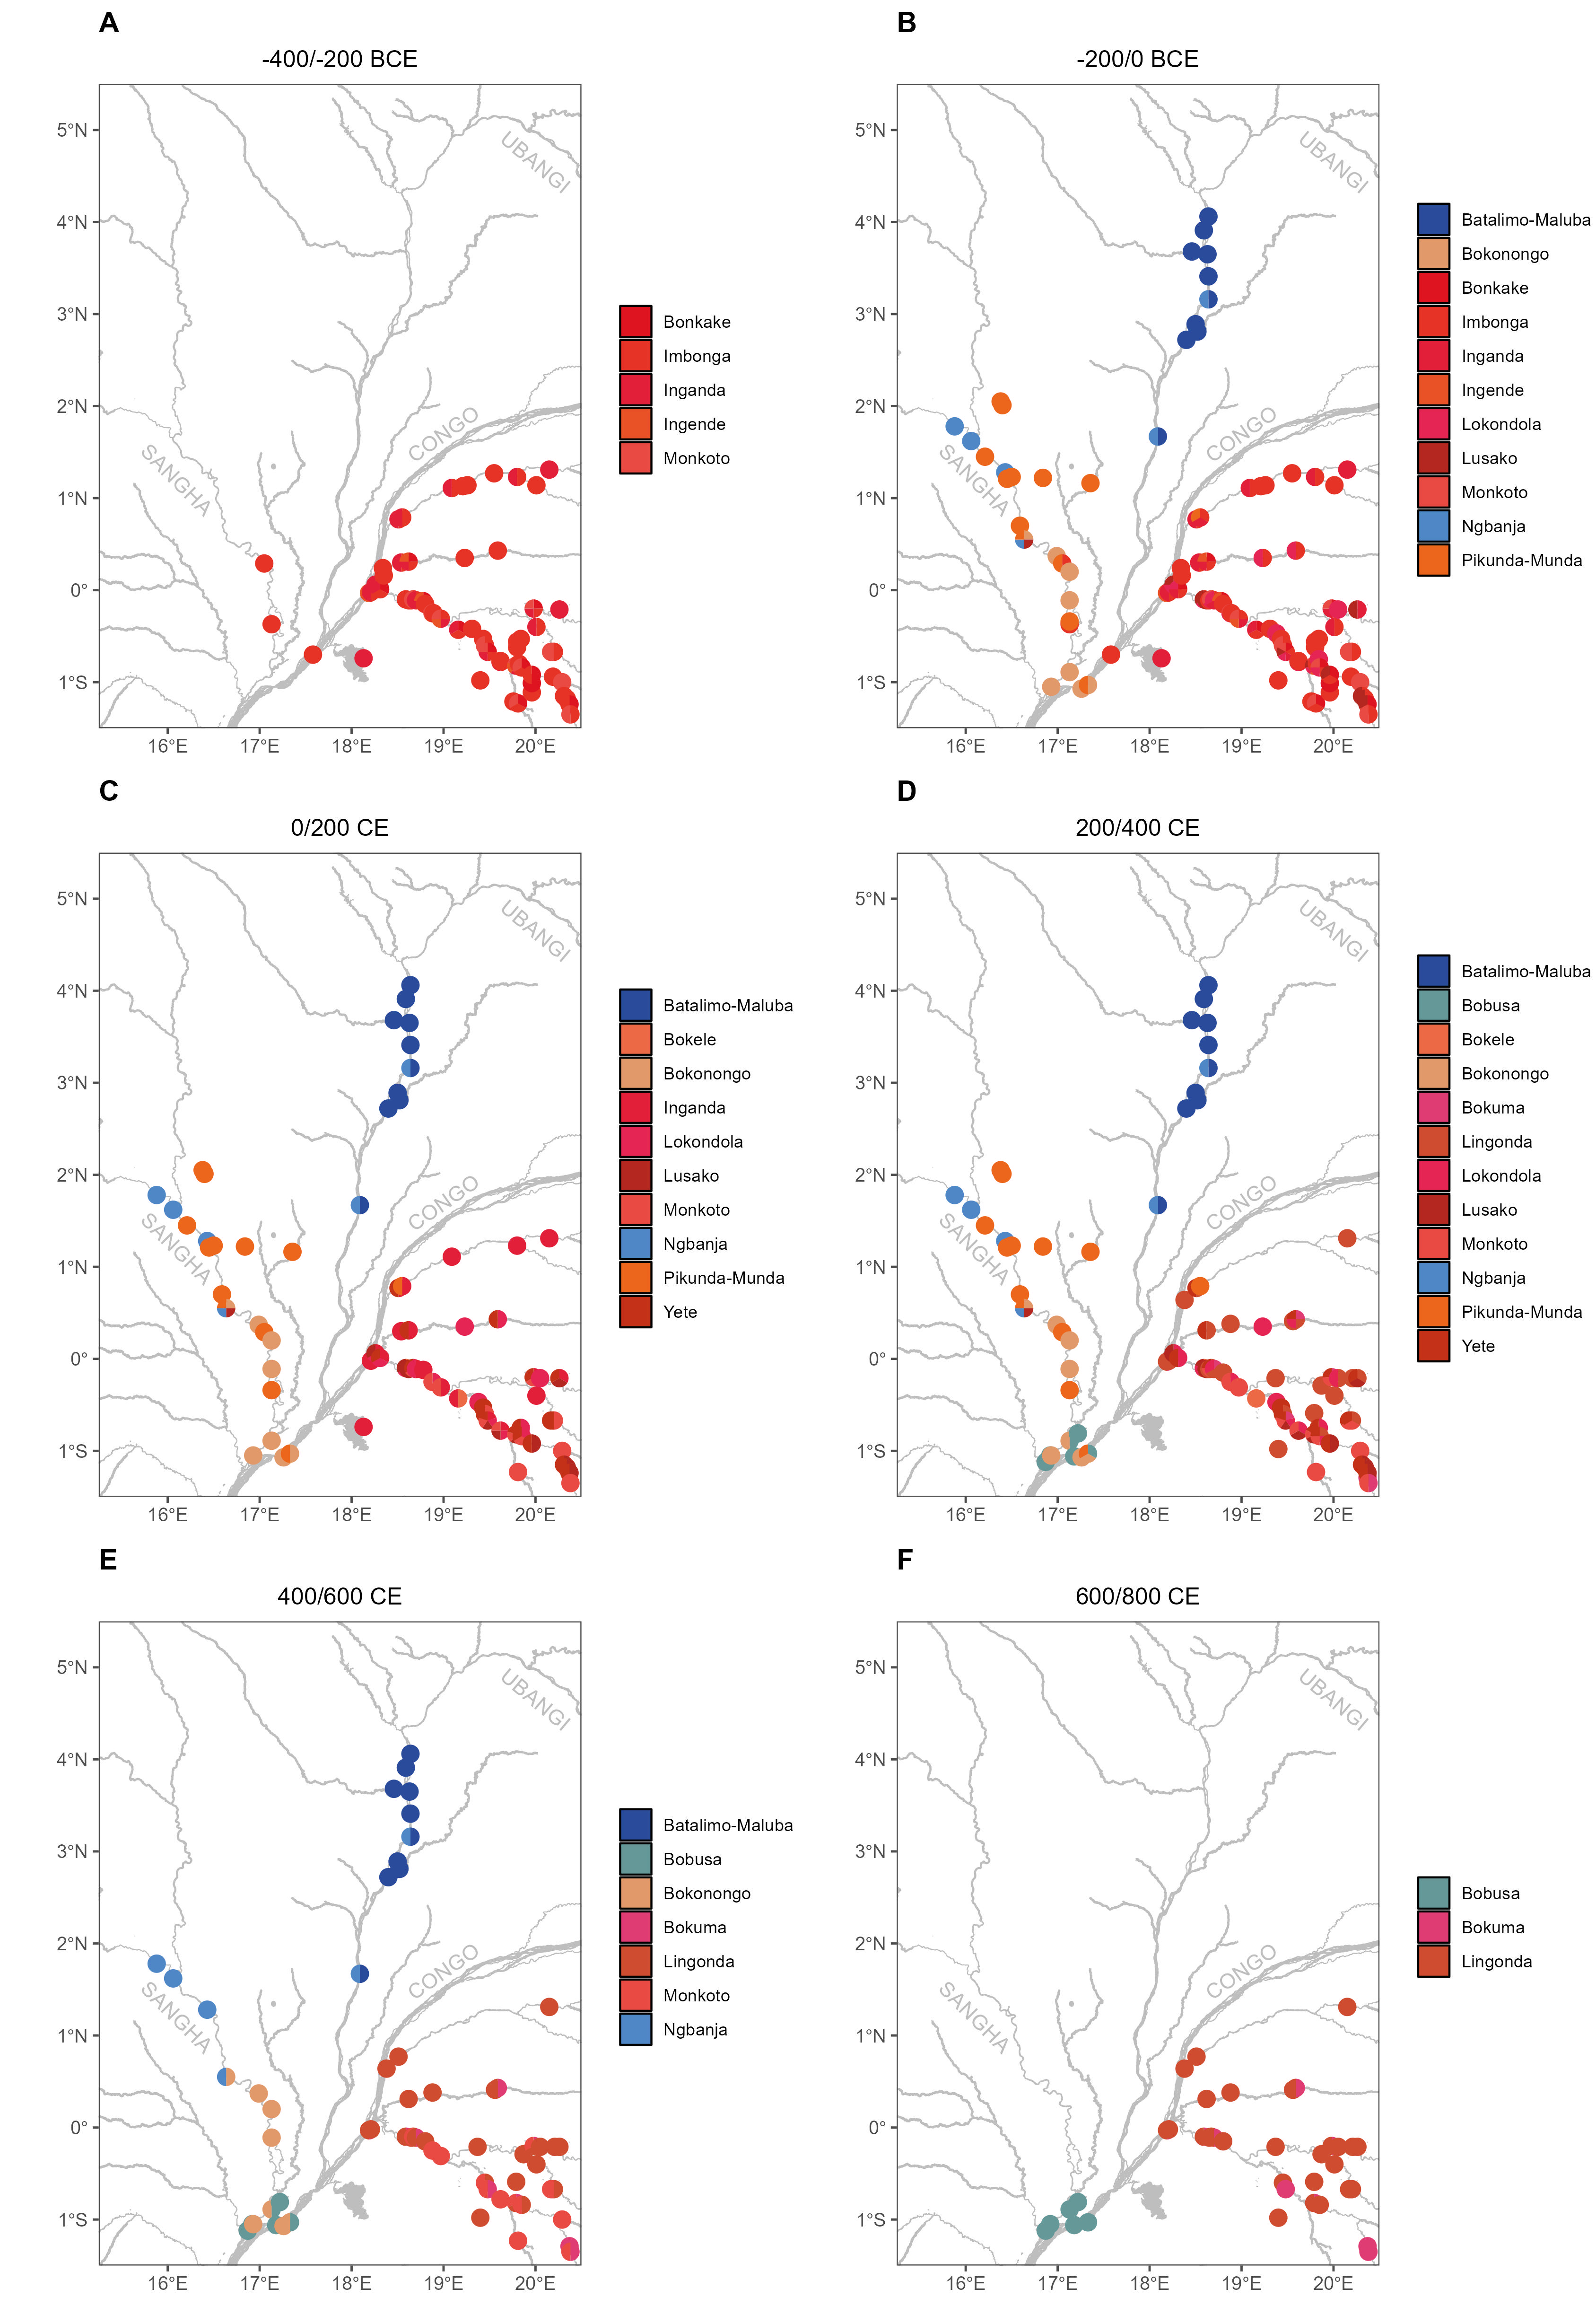
\includegraphics[width=\textwidth]{fig_map_time_slices_1_eia.pdf}
	\caption{Time-sliced maps of occurrences of pottery styles in the northern and western Congo Basin dating between the 4th century BCE to 8th century CE. If multiple contemporaneous pottery styles were recorded at a site, the colored icon is divided following \citet[218--244 Fig.~100--107]{Seidensticker.2021e}. Colors correspond to Fig.~\ref{fig:chrono}.}
	\label{fig:timeslices_1_eia}
\end{figure*}

\subsubsection*{Other Finds}

Several vessels from a partially eroded pit on the banks of the Likwala-aux-Herbes river at kilometer 186 have no comparison in the region in terms of vessel shapes and decorations \citep[165--168, 339--340]{Seidensticker.2021e}. Time constraints during fieldwork only allowed a quick sampling of the pit, obtaining a nearly complete vessel, four larger fragments and 13 smaller sherds (\citeauthor{Eggert.1993} \citeyear{Eggert.1993}, 320 Fig.~16.15; \citeauthor{Seidensticker.2021e} \citeyear{Seidensticker.2021e}, Pl.~76.1--11). A charcoal sample dates this features between the 2nd century BCE to the 3rd century CE (Tab.~\ref{tab:14Cold}: KI-2893). The vessel has a flat base, convex belly, and a slightly elaborated shoulder leading to a concave neck and a flared rim. Its decoration consists of crudely made crossing grooves made with a comb on the shoulder and impressions beneath the rim. Further fragments show similar decorations. Overall, the vessel's shape is substantially different from those of the contemporaneous Pikunda-Munda style. Some aspects of the ceramics superficially resemble a vessel found at Gbadolite on the upper Ubangi river \citep[277--278 Fig.~7]{Eggert.1984}. Loosely similar in terms of vessel shapes, decoration technique and motives is the pottery of the Ngovo group of the lower Congo region \citep[167 Fig.~81]{deMaret.1986,Seidensticker.2021e}.

The Bokonogo style is an interim term for an inventory of 19 vessel units from seven sites, including Pikunda on the middle Sangha river, that show very distinct characteristics: all vessels are either rather tall with convex bellies and concave necks ending in cylindrical rims or bowls with inverted rims \citep[Fig.~\ref{fig:sangha}.4;][120--123]{Seidensticker.2021e}. Decorations consist of grooves beneath the rim and on the neck and shoulders, mainly forming horizontal, chevron or crossing motives. About half of the inventory showed a fabric similar to that of the Pikunda-Munda group, while a quarter showed grog tempering. At the same time, the remainder contained a heterogenous mix of quartz and grog. All finds are surface finds and not associated with any indications of their dating. The only loose comparison in terms of morphological characteristics and decorations can be made towards the Oveng pottery found in north-western Gabon \citep[615--618]{Clist.20042005} and on the island of Corisco (Equatorial Guinea) dating into the 1st to 7th century CE (\citeauthor{Clist.20042005} \citeyear{Clist.20042005}, 555 Fig.~7–14; \citeauthor{GonzalezRuibal.2011} \citeyear{GonzalezRuibal.2011}; \citeyear{GonzalesRuibal.2012}; \citeauthor{SanchezElipe.2015} \citeyear{SanchezElipe.2015}, 217--221; \citeauthor{SanchezElipe.2016} \citeyear{SanchezElipe.2016}, 351--355).

Close to the mouth of the Sangha river, in the very south of the study area, a unique kind of pottery was found that is characterized by predominant grog tempering and small globular pots with short everted rims or convex bowls with slightly inverted rims \citep[Fig.~\ref{fig:sangha}.6--8;][162--165]{Seidensticker.2021e}. This group is named after the site of Bobusa, located near the mouth of the Sangha river. While there are no radiocarbon dates available for this pottery group, some of its characteristics show similarities to pottery found on the Île des Mimosas in Kinshasa \citep[279--280]{Eggert.1984}.

\subsection*{Early Iron Age (200 BCE – 500 CE) in the Northern Congo Basin}

The 1985 survey along the Ubangi river from its mouth into the Congo river south of Mbandaka up to Kouango and along the Lua river (Fig.~\ref{fig:map}) yielded a first glimpse into the variability of ceramics in the northern parts of the Congo Basin. The distribution of pottery groups in the northern Congo Basin is separated into three distinct regional lines of development \citep[183--185]{Seidensticker.2021e}: only along the middle part of the Ubangi river, from around 180 to 240~km upstream of its mouth into the Congo river up to Bangui, pottery dating into the late 1st millennium BCE to 1st millennium CE was uncovered.

\subsubsection*{Batalimo-Maluba style}

In the region between Impfondo and Bangui, henceforth referred to as the middle Ubangi river, the ceramic sequence starts with the Batalimo-Maluba style \citep[75--82]{Seidensticker.2021e}, named after the eponymous sites Batalimo on the lower Lobaye river and Maluba on the lower Lua river (Fig.~\ref{fig:map}). Excavations at Batalimo were conducted by \citet{deBayledesHermens.1975}, Vidal, \citet{Kote.1992} and \citet{Ndanga.2010}. The initial excavation indicated a coexistent of partially polished lithic artifacts and ceramics \citep{Aumassip.1975}. This was not supported by later excavations at the site \citep{Ndanga.2010}, nor excavations at the other eponymous site Maluba \citep{Eggert.1987c}. The pottery of the Batalimo-Maluba style was found at 18 sites, with a core distribution area between Dongo near the mouth of the Lua river and Mokelo, about 30~km downstream of Bangui. The most southern find was uncovered at Ngbanja near Impfondo \citep[Fig.~\ref{fig:timeslices_1_eia}B--E;][81 Fig.~25]{Seidensticker.2021e}. Only in Batalimo and Maluba excavations yielded pottery of this style. The other sites associated with this group originate from surface finds. Available radiocarbon dates and one thermoluminescence date (OxTL-154a-4), indicate that the Batalimo-Maluba pottery dates between the 2nd century BCE and 6th century CE \citep[Fig.~\ref{fig:chrono}; S1; Tab.~S1;][80 Fig.~28]{Seidensticker.2021e}. 

Batalimo-Maluba pottery is characterized by well-structured, flat-based globular pots and wide-mouthed bowls that are elaborately decorated using cross-hatching, impression motifs and incised or grooved lines organized in alternating horizontal and vertical zones (Fig.~\ref{fig:ubangi}.1--3; \citeauthor{Eggert.1993} \citeyear{Eggert.1993}, 306--308; \citeauthor{Seidensticker.2016b} \citeyear{Seidensticker.2016b}, 118; \citeyear{Seidensticker.2021e}, 75--82).

\begin{figure*}[!tb]
	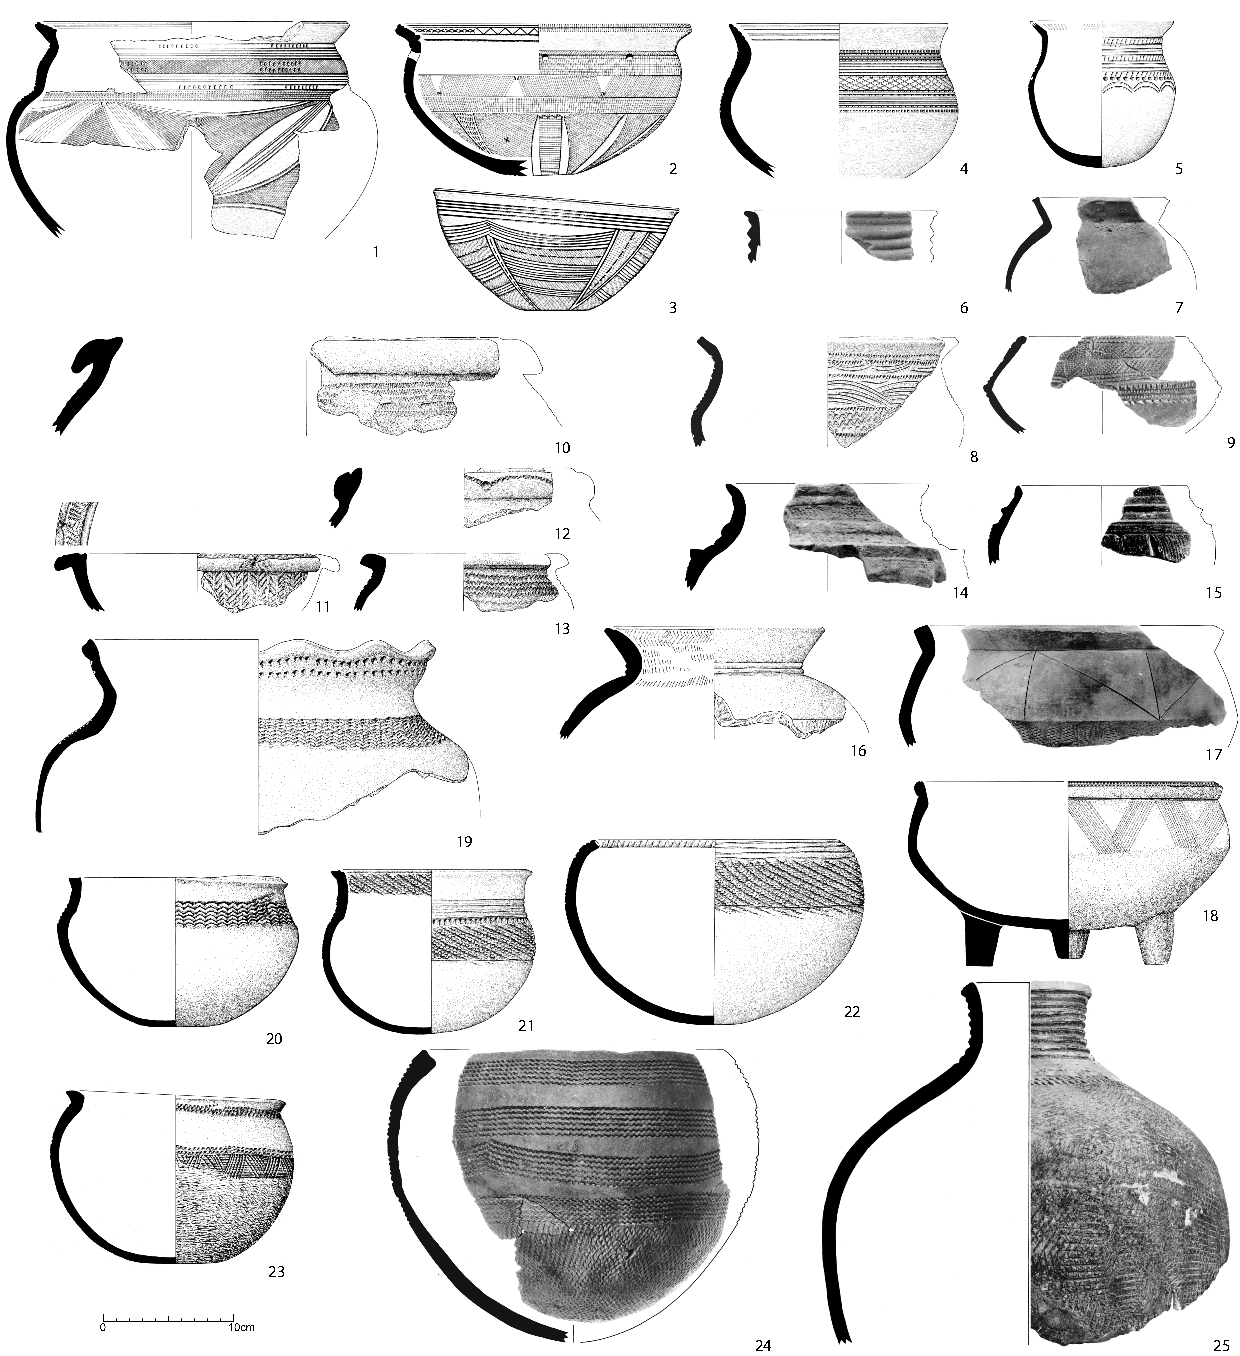
\includegraphics[width=\textwidth]{Ubangi_Typen.pdf}
	\caption{Ceramic vessels from the northern Congo Basin -- along the rivers Ubangi and Lua -- that are representative for the following pottery styles: 1--3) Batalimo-Maluba; 4--5) Ngbanja; 6--7) Bobulu; 8--9) Mokelo; 10--13) Motenge-Boma; 14--15) Bondongo; 16) Mbandaka; 17--18) Bokwango; 19--20) Dama; 21--22) Mbati-Ngombe; 23) Bangui; 24) Kpetene; 25) Botendo \citep[75--114,172--181]{Seidensticker.2021e}.}
	\label{fig:ubangi}
\end{figure*}

\subsubsection*{Nbganja style}

Closely related to the Batalimo-Maluba style is the Ngbanja style, which shares similar general characteristics \citep[82--86]{Seidensticker.2021e}. The primary vessel types are globular or slightly ovaloid pots or beakers with everted rims (Fig.~\ref{fig:ubangi}.4--5). Decorations are based on grooves and impressions, and while they show similar motives as the Batalimo-Maluba style, they are restricted to the neck or inside of the rim.

Ngbanja pottery is strongly related to the Batalimo-Maluba style, and Eggert (\citeyear{Eggert.1987c}, 141) suggested it as a predecessor of the Batalimo-Maluba group. Besides the stylistic connections, the only chronological fixpoint for the Ngbanja style is a sherd of this style found in the deep pit at Pikunda (Sangha river). Two radiocarbon dates (Tab.~\ref{tab:14Cold}: KI-2877; Tab.~\ref{tab:14Cnew}: RICH-30864) date the feature to the second half of the 1st century BCE to the late 3rd century CE. The sherd exhibits a coarse fabric instead of the delicate fabric common to the Pikunda-Munda style, and its decor consists of a ledge with comb impressions on it. A nearly matching sherd was found during surveys at Ngbanja on the middle Ubangi river \citep[83 Fig.~26.7--8]{Seidensticker.2021e}. At Pikunda, this sherd must be considered a foreign but contemporaneous type within the closed Pikunda-Munda inventory. Three other sherds with coarse fabric and a decoration different from the Pikunda-Munda style were also found. These associations allow for the possibility that Ngbanja pottery is contemporaneous not only to Batalimo-Maluba pottery but also to the Pikunda-Munda style and dates between the 2nd/1st century BCE and the 5th/6th century CE (Fig.~\ref{fig:chrono}; \ref{fig:timeslices_1_eia}B--E).

\subsection*{Hiatus (500--1000 CE) in the Congo Basin}

In both regions, inventories dating between the end of the 6th century to the early 10th century CE are currently unknown, leaving a gap within the regional sequences of at least 300 years (Fig.~\ref{fig:chrono}; \ref{fig:timeslices_1_eia}F--\ref{fig:timeslices_2_lia}A; S1). A detailed review of chronological indicators for the 32 pottery styles described by Wotzka (\citeyear{Wotzka.1995}, 59--212) revealed a similar pattern: no pottery could be dated between the end of the Bokuma and Lingonda styles, which end towards the end of the 7th centuries CE, and the onset of the widespread Bondongo style at the beginning of 12th century CE (Fig.~S1; Tab.~S2).

In the north-eastern Congo Basin, around Kisangani (Fig.~\ref{fig:map}), a similar interruption between ceramics designated to the Early and Middle Pottery Phase and styles pertaining to the Late Iron Age has been observed \citep[Fig.~\ref{fig:chrono}; S1]{LivingstoneSmith.2017}. Technological analyses of the shaping techniques revealed a distinction as well: the pottery of the Early and Middle phases is exclusively shaped via a drawing of a ring technique, while all Late Iron Age pottery is shaped by pounding in a concave mold. Only certain stages of the \textit{chaînes opératoires} of the Late Iron Age ceramics still adhere to principles followed during earlier times, indicating a certain continuity (pers. comm. Livingstone-Smith 2021).

Two recent papers firmly established the supra-regional pattern of putative demographic changes in Central Africa during the past three millennia, both showing strong empirical evidence for a setback in human activity between the 6th to 10th century CE \citep{deSaulieu.2021a,Seidensticker.2021}. These independent results have been critically reviewed by \citet{Clist.2023a}.

\subsection*{Late Iron Age (1000--1850 CE) in the Western Congo Basin}

After the interruption of pottery sequences during the 6th to 10th century CE, ceramics re-appear within the archaeological inventories of the region in the 10/11th century CE (Fig.~\ref{fig:chrono}; \ref{fig:timeslices_2_lia}A--B; S1). During the late Iron Age in the western Congo Basin, a clear distinction appears between pottery styles associated with the adjacent Inner Congo Basin and an independent stream summarized as Ngoko style tradition.

\subsubsection*{Ngombe style}

The re-emergence of ceramics in the western Congo Basin at the onset of the Late Iron Age is marked by the Ngombe style \citep[125--128]{Seidensticker.2021e}, which is rooted in the Equator-Co tradition of the Inner Congo Basin \citep[222 Fig. 4]{Wotzka.1995}. The ceramics of this type are found mainly on the lower Sangha river, with the eponymous site of Ngombe constituting the northernmost extension of its distribution area \citep[127 Fig. 54]{Seidensticker.2021e}. In total, 56 vessel units from 15 sites are associated with the Ngombe style. They are similar to the Longa and Mbandaka styles \citep[121--128, 139--143]{Wotzka.1995} of the Inner Congo Basin but show equally independent characteristics. The defining inventory of the Ngombe style was discovered in a partially eroded pit at the eponymous site on the middle Sangha river \citep[305--306]{Seidensticker.2021e}. It yielded an inventory of two plates, a big bowl, and a carinated bowl, all surrounded by fragments of a large vessel with a convex belly, a tapered shoulder and a short, flared rim \citep[Fig.~\ref{fig:sangha}.10--12;][Pl. 42.15--44.2]{Seidensticker.2021e}. The Ngombe style shows only rounded bases. Decorations consist of grooves and impressions on the upper parts of the vessels. A new radiocarbon date obtained off a food crust from the bottom of the main vessel found at Ngombe dates into the late 12th to mid 13th century CE (RICH-30867; Tab.~\ref{tab:14Cnew}). This corroborates the previously proposed age of this pottery in relation to the Mbandaka and Longa styles of the Inner Congo Basin \citep[Fig.~\ref{fig:chrono}; \ref{fig:timeslices_2_lia}B--C; S1; Tab.~S1;][126--128]{Seidensticker.2021e}. 

\begin{figure*}[!tbp]
	\centering
	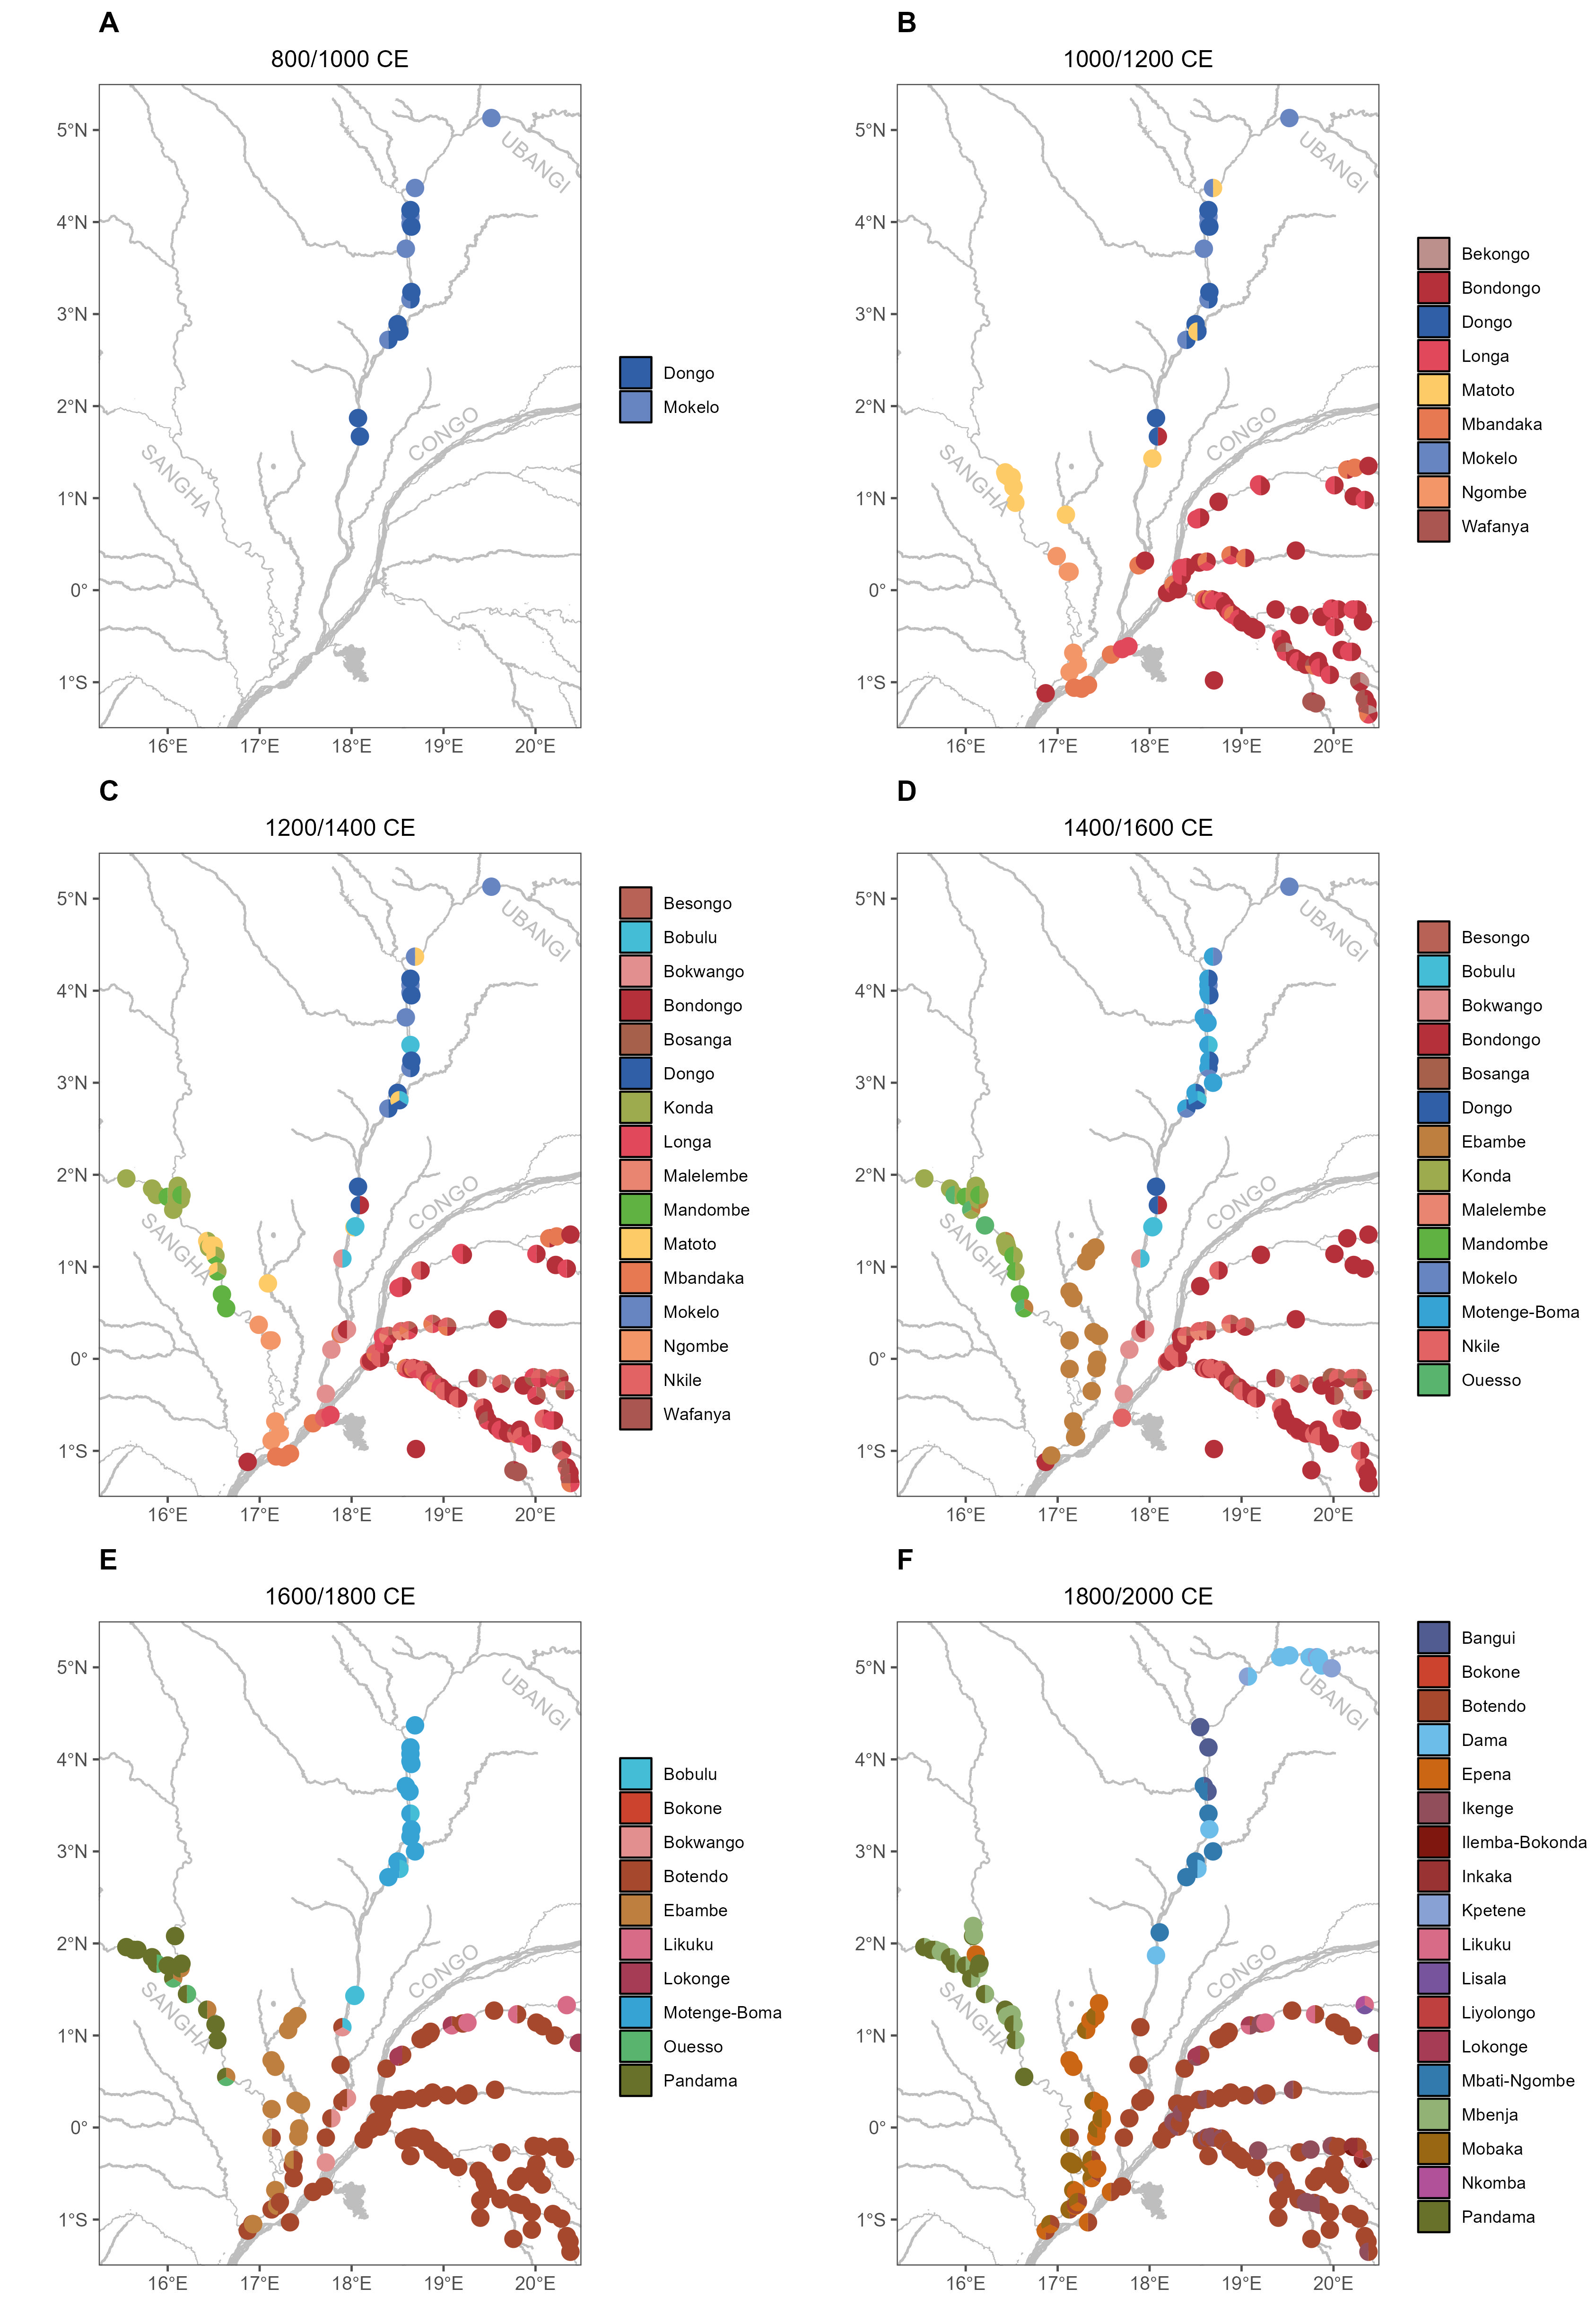
\includegraphics[width=\textwidth]{fig_map_time_slices_2_lia.pdf}
	\caption{Time-sliced maps of occurrences of pottery styles in the northern and western Congo Basin dating younger than the 9th century CE. If multiple contemporaneous pottery styles were recorded at a site, the colored icon is divided following \citet[218--244 Fig.~100--107]{Seidensticker.2021e}. Colors correspond to Fig.~\ref{fig:chrono}.}
	\label{fig:timeslices_2_lia}
\end{figure*}

\subsubsection*{Ebambe and Epena styles}

Modern pottery production in the western Congo Basin shows two styles being present along the Likwala-aux-Herbes river: upstream dominates the Epena style, while downstream, the Ebambe style is more present, but with vessels of both styles being found along the entire length of the river \citep[131--141]{Seidensticker.2021e}. Only the Ebambe style has been found along the lower Sangha river. A potter in Boleko, on the lower Likwala-aux-Herbes river, was still producing pottery of the Ebambe style in 1987 using a drawing of a lump technique combined with additional coiling for the neck \citep{Eggert.inVorb.}. Diagnostic  shapes include tall vessels with tapered necks, bottles with think necks and bowls with parallel rims \citep[Fig.~\ref{fig:sangha}.13--14;][132 Fig.~57]{Seidensticker.2021e}. All vessels of the Ebambe style show flat bases. A diagnostic feature of the Ebambe style is the consistent use of \textit{banfwa-nfwa} decor on nearly all parts of the vessel, including occasionally the inside of the rims. \textit{Banfwa-nfwa} is the characteristic decoration technique employed by potters at Ikenge \citep[399]{Eggert.1980c} and can be found on most of the pottery of the Inner Congo Basin after the onset of the Late Iron Age \citep[109--111]{Wotzka.1995}. It is created by whipping the leather hardened clay with the narrow side of a chip made from the rib of a palm leaf, leaving short, mostly lancet-shaped impressions \citep[Fig.~\ref{fig:sangha}.13--14; \ref{fig:ubangi}.16,25;][386 Ftn.~5]{Eggert.1980b}.

A rich inventory of Ebambe style vessels was excavated in Munda on the upper Likwala-aux-Herbes river \citep[311--321]{Seidensticker.2021e}. New radiocarbon dates on food crusts from two vessels found within the pit (Tab.~\ref{tab:14Cnew}: RICH-30865--RICH-30866) corroborate the existing convention date (Tab.~\ref{tab:14Cold}: KI-2884). All three dates cover the 16th century CE onwards.

The pottery produced at Epena on the upper Likwala-aux-Herbes river shares similar morphological features with the Ebambe style, especially their flat bases and tall vessels with tapered necks \citep[Fig.~\ref{fig:sangha}.16--17;][137--141]{Seidensticker.2021e}. Production was documented in 1995 by Léopold Mpika Ngoma (\citeyear{MpikaNgoma.1996}, 25--33). Epena ceramics -- labeled 'Jeke' in \citet[119 Fig.~6.3]{Seidensticker.2016b} -- were shaped via drawing of superimposed rings. Most vessel shapes show relatively straight walls with slight tapering on the largest diameter and everted rims \citep[138 Fig.~60]{Seidensticker.2021e}. Decorations are usually reserved for the shoulder and neck area. The rims are regularly undecorated, and -- unlike the Ebambe pottery -- bellies are not decorated with \textit{banfwa-nfwa}. There are no chronological indicators for the onset of the Epena style available.

\begin{figure*}[!tb]
	\centering
	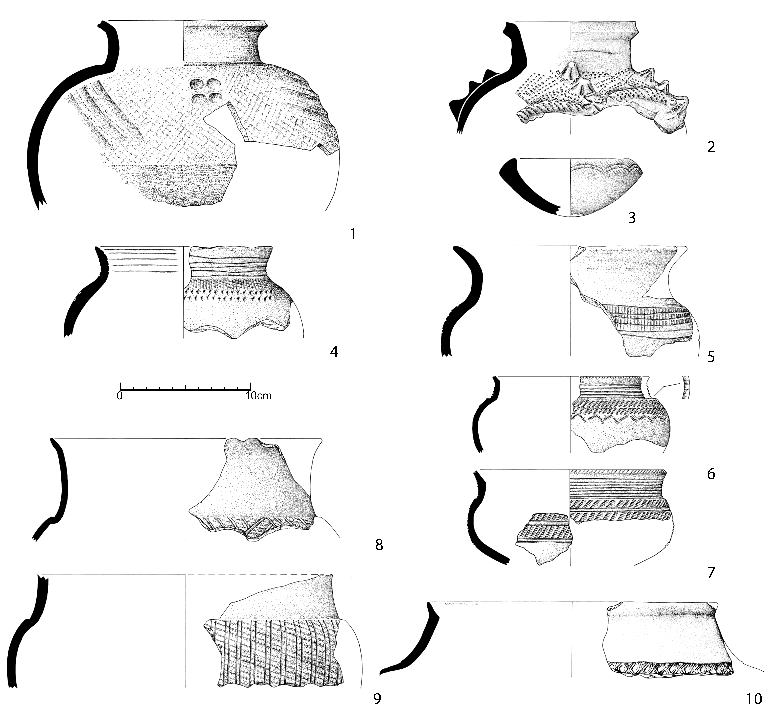
\includegraphics[width=.6\textwidth]{Ngoko-Trad_Typen.pdf}
	\caption{Ceramic vessels of the Ngoko style tradition -- along the rivers Ngoko and Sangha -- that are representative for the following pottery styles: 1--3) Mandombe; 4--5) Konda; 6--7) Ouesso; 8--9) Pandama; 10) Mbenja \citep[145--162]{Seidensticker.2021e}.}
	\label{fig:ngoko}
\end{figure*}

\subsubsection*{Ngoko style tradition}

Between the 13th to 15th centuries CE, a set of ceramics emerged that showed no connection to the Equator-Co tradition and constituted an independent style tradition (Fig.~\ref{fig:ngoko}). Two out of the five pottery styles forming the Ngoko style tradition are dated: the Mandombe style \citep[145--148]{Seidensticker.2021e}, which was defined after the inventory excavated in the upper pit at Pikunda, dates into the 13th to 15th century CE (Tab.~\ref{tab:14Cold}: KI-2891), and the Mbenja style \citep[158--162]{Seidensticker.2021e}, which represents the modern pottery along the upper Sangha and the Ngoko. The other three styles that are part of the Ngoko style tradition can -- thus far -- only be dated relative to these two groups \citep[121--123 Fig.~6.5]{Seidensticker.2016b}: the Pandama style \citep[155--158]{Seidensticker.2021e} shows considerable similarities with the modern Mbenja pottery, the Quesso style \citep[152--155]{Seidensticker.2021e} shows similarities to the Pandama style, and the Konda group \citep[148--152]{Seidensticker.2021e} shows similarities to the styles Mandombe and Pandama respectively. The proposed order of these pottery styles starts in the 13th to 15th century CE with the Mandombe style, followed by the Kondo group and the Ouesso group, which in turn are surpassed by the Pandama style, which links to the modern Mbenja pottery.

All styles within the Ngoko style tradition share similar main vessel types: pots with convex bellies, concave necks, and short, everted rims. While decorations in the Mandombe style are based on grooves, often using a comb, and comb impressions, the lower halves of the vessels are consistently roughed up by a slurry or slip (Fig.~\ref{fig:ngoko}.1--3). A diagnostic property are plastic decorations, such as knobs and ledges, that can only be found among vessels of the Mandombe style. While relying on grooves and impressions, the succeeding Konda style shows no elevated decoration (Fig.~\ref{fig:ngoko}.4--5). The Ouesso pottery shows decorations made through grooving and comb impressions, similar to the Konda pottery (Fig.~\ref{fig:ngoko}.6--7). At the same time, the shape of the rims is similar to the Pandama style. The decorations of Pandama pottery are based on knotted strip, twisted string, and alternate knotted strip roulettes, which are sometimes superimposed by grooves (Fig.~\ref{fig:ngoko}.8--9). Roulette decoration was previously observed only in some vessel units associated with the styles Mandombe and Konda. This indicates a slow and staged introduction of roulette within the developed system of the Ngoko style tradition \citep[120--123]{Seidensticker.2016b}. Within the modern Mbenja style, vessel shapes become more heterogeneous, while the shape of the rims persist. Concerning decorations, Mbenja pottery shows carved roulette only and decor is restricted to a single band on the vessel’s shoulder (Fig.~\ref{fig:ngoko}.10). None of the ceramics associated with the Ngoko style tradition show fabrics indicative of the usage of fine riverine clays \citep{Seidensticker.2020}. Sherds contain substantial quantities of quartz and organic temper. Pottery of the Mandombe style excavated at Pikunda, and modern pottery produced in Pikunda in 1987, decorated with knotted strip roulette, was produced using coiling. All these styles show inherent commonalities and, at the same time, substantial differences to any pottery linked to the Equator-Co style tradition of the Inner Congo Basin \citep{Wotzka.1995}. The fieldwork of the \textit{River Reconnaissance Project} in 1987 only uncovered the southern margins of the Ngoko tradition, which reached as far south as Pikunda on the middle Sangha river (Fig.~\ref{fig:timeslices_2_lia}C--F). Its upstream or northern extent can only be revealed during future fieldwork in the south-east of Cameroon and the south-west of the Central Africa Republic respectively.

\subsection*{Late Iron Age (1000--1850 CE) in the Northern Congo Basin}

During the younger part of the pottery sequence in the northern Congo Basin the three-way split of regional ceramic development persists: on the lower part of the river, up to 180 to 240~km upstream, all observed ceramics are part of the Equator-Co tradition of the Inner Congo Basin. Inventories from sites in that region are dominated by the newly described Bokwango style and the already established styles Bondongo, Mbandaka, and Botendo \citep[96--98, 172--181]{Seidensticker.2021e}. The area further upstream, up to Bangui, showed a complex set of pottery styles described below. Upstream of Bangui, only very young pottery has been identified as of yet. A key characteristic of the pottery styles pertaining to the Late Iron Age along the Ubangi river is the introduction of roulette decoration in an equally staged and slow process as in the Ngoko style tradition. 

While excavations in this area are rare, only pits with Batalimo-Maluba pottery at Maluba were sufficiently excavated during the \textit{River Reconnaissance Project}, there are no adequately documented inventories known thus far that yielded pottery dating into the Late Iron Age. Therefore, all lines of reasoning are based on stylistic developments within survey inventories. Modern pottery production documented at four sites on the middle and upper Ubangi river are the only points of reference.

At Mbati-Ngombe on the middle Ubangi river, the production of short-necked vessels and bowls with round bases (Fig.~\ref{fig:ubangi}.21--22) shaped via coiling was observed \citep[109--121]{Seidensticker.2021e}. Bowls show inverted rims, while the vessels usually have a short cylindrical neck and very short, everted rim. Most distinctive is the systematic decoration of vessels of the Mbati-Ngombe group using either knotted strip, twisted string, or alternated knotted strip roulettes \citep[88--105]{LivingstoneSmith.2010b} in a single band below the rim or occasionally on the inside of the rim.

Further upstream, ceramic vessels were produced at Dama 1, Sidi and Boduna by pounding in a concave mold \citep[69 Ftn.~101]{Seidensticker.2021e}. Dama style pottery \citep[104--109]{Seidensticker.2021e} consists of either smaller pots with rounded bases and short everted rims but without a defined neck area or substantially bigger vessels with pronounced convex shoulders and everted rims (Fig.~\ref{fig:ubangi}.19--20). The primary means of decoration within the Dama style are carved roulettes, consistently applied in a single band on the vessel’s shoulder. Only rarely is the roulette accompanied by grooves or impressions.

The Kpetene style summarizes a set of ethnographic vessels whose production was not documented. This style is comprised of ovaloid vessels and bowls with round bases that are extravagantly decorated with multiple bands of carved roulette \citep[103--105]{Seidensticker.2021e}. Near Bangui, modern vessels with flat bases and a decoration not relying on roulettes are observed \citep[112--114]{Seidensticker.2021e}. This group, named after the capital of the Central African Republic, shows systematic roughing up of the lower parts of the vessels with \textit{banfwa-nfwa}. In contrast, the upper parts are decorated with multiple bands of impressions and grooves (Fig.~\ref{fig:ubangi}.24).

The most distinctive style among the precursors of these modern productions is the Motenge-Boma group \citep[99--103]{Seidensticker.2021e}, first discovered by Van Noten (\citeyear{vanNoten.1978}, 75, \citeyear{vanNoten.1982a}, 69, Fig.~40). The vessels of the Motenge-Boma group show convex bellies, no pronounced neck areas and, most importantly, a particular variety of rim shapes (Fig.~\ref{fig:ubangi}.10--13). Often, the usually straight or slightly inverted rims show thick ledges. The spectrum of vessel shapes within the Motenge-Boma group also includes convex bows with thickened rims. A clear marker of the Motenge-Boma pottery is a decoration based on bands of carved or, in some cases, knotted strip roulette in combination with grooves and impressions on the bellies and shoulders of vessels. The rims are often also decorated similarly. No new pointers for the dating of the Motengo-Boma pottery have been obtained as studied ceramics of this style were found entirely as surface finds. Thus, until excavations uncover inventories pertaining to this style as well as datable material, the age of the Motenge-Boma pottery can only be estimated to be somewhere in the second half of 2nd millennium CE as suggested by Van Note (\citeyear{vanNoten.1982a}, 69). The detailed surveys of 1985 could demarcate the distribution of this pottery along the Ubangi river quite well. Motenge-Boma ceramics are only found from the mouth of the Lua river in the south to Bangui in the north \citep[Fig.~\ref{fig:timeslices_2_lia}D--E;][102 Fig.~37]{Seidensticker.2021e}.

Evidence for pottery dating between the end of the Batalimo-Maluba style in the 6th century CE (Fig.~S1; Tab.~S1) and the onset of the Motenge-Boma group is scarce. The styles Dongo, Mokelo and Bobulu \citep[Fig.~\ref{fig:chrono};][86--95]{Seidensticker.2021e} are noteworthy as they date potentially between the mid of the 1st millennium CE and the middle of the 2nd millennium CE. The most diagnostic among these is the Mokelo pottery, distributed between the mouth of the Lua river and the bend of the Ubangi river further upstream. Its vessels often show tapered profiles (Fig.~\ref{fig:ubangi}.8--9). While carved roulette decoration is occasionally present, the bulk of its decors is achieved utilizing incisions and bands of comb impressions.

Notably, no ceramics dating to before the 10th century CE were found along the lower stretches of the Ubangi river, south of Impfondo. All finds from that region pertain to pottery styles known from the Inner Congo Basin, such as Bondongo, Mbandaka, and Botendo \citep[Fig.~\ref{fig:ubangi}.14--16,25;][172--181]{Seidensticker.2021e}, with the only exception being the newly described Bokwango style \citep[Fig.~\ref{fig:ubangi}.17--18;][96--99]{Seidensticker.2021e}. The ceramics of this group are an off-shoot for the Equator-Co style tradition \citep{Wotzka.1995}. The lower halves of Bokwango vessels are decorated with \textit{banfwa-nfwa}, as is typical for styles from the Inner Congo Basin dating into the Late Iron Age but showing slightly tapered profiles.

\section*{Discussion}

\subsection*{Settlement History of the Congo Basin}

The results from the northern and western parts of the Congo Basin presented here complement the available data on the settlement history of the Inner \citep{Wotzka.1995} and north-eastern Congo Basin \citep{LivingstoneSmith.2017}, enabling a synopsis of the settlement history of the region as a whole \citep[218--244]{Seidensticker.2021e}. The earliest pottery group known within the entire Congo Basin thus far is the Imbonga style, dating into the 4th to 2nd century BCE (Fig.~\ref{fig:chrono}; S1; Tab.~S1) that is found within the western half of the \textit{Cuvette central} \citep[Fig.~\ref{fig:timeslices_1_eia}A;][59--68]{Wotzka.1995} as well as at two sites along the lower Sangha river.

The Imbonga style differentiates into multiple groups that still inherit substantial morphological and decoration characteristics in the following phase, starting in the 3rd and 2nd century BCE \citep[219--224]{Seidensticker.2021e}. Initially, the later individually described styles Bonkake, Ingende and Inganda \citep[Fig.~\ref{fig:chrono}; S1; Tab.~S1;][68--84]{Wotzka.1995} were conceptualized as part of a broader ‘Imbonga horizon’ \citep{Eggert.1983}. During this time, the settled area in the Inner Congo Basin slightly expanded upriver along the lower Tshuapa, up to the region of the modern town of Boende, and on the lower Luilaka (Fig.~S2B). The development of ceramic styles in the Inner Congo Basin around the turn of time is characterized by differentiation and regionalization, with many of the successors of the Imbonga style being only distributed along certain tributaries of the Congo river.

Also within this time period, the initial phase of pottery-producing communities emerged in the north-eastern parts of the Basin, in the vicinity of Kisangani \citep[Fig.~S2A;][]{LivingstoneSmith.2017}. The pottery of the Early Phase dates between the 2nd century BCE and 1st century CE (Fig.~\ref{fig:chrono}; S1; Tab.~S1). \citet[110,115]{LivingstoneSmith.2017} propose a relation of this pottery to the contemporaneous Imbonga style of the Inner Congo Basin, especially regarding the use of similar decorative techniques. In a critical review it must be noted that the pottery of the Early Phase \citep[112 Fig.~24]{LivingstoneSmith.2017} lacks systematic rocker zig-zag on the bottom parts of vessels as well as raised decorations such as ledges or ridges, vessels shows no pronounced shoulders, all primary characteristics of the Imbonga style \citep[170 Fig.~84.1--20]{Seidensticker.2021e}. Pottery of the Early Phase is still attested until the 1st century CE, while the Middle Phase pottery already commences \citep[Fig.~\ref{fig:chrono}; S1; Tab.~S1;][]{LivingstoneSmith.2017}.

In the 2nd to 1st century BCE pottery-producing communities emerge in the western and northern Congo Basin: along the Sangha and Likwala-aux-Herbes rivers, the Pikunda-Munda style and along the middle Ubangi river, on the northern fringes of the rainforest, the Batalimo-Maluba (Fig.~\ref{fig:chrono}; S1; Tab.~S1) and the Ngbanja styles can be found (Fig.~\ref{fig:timeslices_1_eia}B). It is essential to state that these groups share no fundamental commonalities with the pottery of the Inner Congo Basin and must be regarded as distinct and individual lines of development. Based on preliminary technological analyses, a connection to the Inner Congo Basin's contemporaneous ceramics can only be postulated for the Pikunda-Munda group. Ceramics within the western and Inner Congo Basin appear to have been shaped in either a drawing of a lump or a ring technique. These ceramics have yet to be differentiated, especially regarding used clays and the lack of tempering of the clays \citep{Seidensticker.2020}. 

The first half of the 1st millennium CE sees a continuation of the described patterns. In the Inner Congo Basin, multiple interrelated styles with only regional distribution areas emerge (Fig.~S2C--D). It should be remarked that during this time, a slight retreat of settlement activity is discernible, with substantially fewer sites compared to the centuries BCE being known along the Lulonga and Lopori rivers \citep[224]{Seidensticker.2021e}. This plateauing of settlement activity led to the setback in human activity visible throughout Central Africa that continued until the 10th century CE \citep{Seidensticker.2021}.

Within the entire Congo Basin, only very few dated sites point to the presence of pottery-producing communities between the 7th to 10th centuries CE (\citeauthor{Seidensticker.2021e} \citeyear{Seidensticker.2021e}, 225--231; \citeauthor{Seidensticker.2021} \citeyear{Seidensticker.2021}, Fig. S4). The two predominant styles in the western and northern Congo Basin, the Pikunda-Munda and Batalimo-Maluba groups, end between the 4th to 6th century CE at the latest (Fig.~S1; Tab.~S1). The available dates for the Middle Phase pottery in the Kisangani region indicate that it ended around the same time. The earliest evidence for the Ilambi style, clearly pertaining to the younger Iron Age, dates to the 8th century CE. It must be stressed that this early date is challenged by another date also associated with the Ilambi style, dating into the 15th to 17th century CE, leaving a considerable discrepancy \citep[98 Tab.~1]{LivingstoneSmith.2017}.

Substantial human activity is attested for again by significant increases in sites yielding pottery dating to the 11th century CE and younger. Among these are the widely distributed Bondongo and Longa styles \citep[Fig.~\ref{fig:chrono}; S1; Tab.~S1;][121--139]{Wotzka.1995}. While these groups are distributed across nearly all parts of the Inner Congo Basin that was surveyed during the \textit{River Reconnaissance Project}, and in the case of the Bondongo group also along the lower Ubangi river, they are immediately followed by a distinct development of regional traditions (\citeauthor{Wotzka.1995} \citeyear{Wotzka.1995} 221--223; \citeauthor{Seidensticker.2021e} \citeyear{Seidensticker.2021e}, 231--244; \citeauthor{Seidensticker.2021} \citeyear{Seidensticker.2021}, 3--5). Along the lower Sangha river, the newly dated Ngombe group (Tab.~\ref{tab:14Cnew}) reflects an uptick in human activity. Starting in the 13th century CE, new components of pottery production commence along the Ngoko river and upstream parts at the Sangha river. These new elements form the foundation for the newly described Ngoko style tradition, whose onset is marked by the emergence of the Mandombe style. This group is later followed by at least three more pottery styles that lead directly into the modern potters’ production in the area. Along the Likwala-aux-Herbes river, re-settlement is only attested for starting in the 16th century CE, documented by newly obtained radiocarbon dates for ceramics of the Ebambe style (Tab.~\ref{tab:14Cnew}: RICH-30866). Within a similar time falls the Motenge-Boma style found along the middle Ubangi river. It is putatively preceded by the poorly attested Dongo, Mokelo, and Bobulu groups. The introduction of roulette decoration within the Ngoko style tradition, as well as among the groups on the middle Ubangi river, while being an easily observable maker, cannot be described as a watershed event but rather a process of slow adaption \citep[120--123]{Seidensticker.2016b}. Similarly to these regions, roulette decoration becomes a prime marker of younger pottery styles in the Kisangani region \citep{LivingstoneSmith.2017}. 

\subsection*{Refuting the "Sangha River Interval" (SRI) Hypothesis}

The putative origin of ceramic-producing communities starting to settle in the Congo Basin in the 4th century BCE remains elusive. Linguistic studies propose rapid migrations through the rainforest \citep{Currie.2013,Whiteley.2019,Koile.2022} and suggest that the region of the Sangha river, in the western Congo Basin (Fig.~\ref{fig:map}), played a crucial role as a potential 'gateway' through the equatorial rainforest of the Congo Basin \citep{Grollemund.2015,Bostoen.2015,Grollemund.2023}. In consequence, putative Bantu-speaking migrants are deemed to have followed a savannah-corridor, determined by the Sangha River Interval (SRI), in the latter half of the 1st millennium BCE \citep{Grollemund.2015,Bostoen.2015}. This hypothesis is brought forward based on statistical analyses of present-day languages and attempts to integrate archaeological data into the outcome of these statistical analyses against the background of an ecologically identified "forest perturbation" \citep[356]{Bostoen.2015} during the Late Holocene Rainforests Crisis (LHRC) \citep{Vincens.1994,Elenga.1996,Raynaud-Farrera.1996,Maley.1998b,Vincens.1998,Maley.2004,Ngomanda.2009,Sangen.2009,Giresse.2020}. 

The unique composition of the region along the Sangha river \citep[cf. "W\&E margins" in][7 Fig.~3A]{Philippon.2019}, linking plant and animal species from the Sudanian and Zambezian savannas, was first brought forward in René \citet{Letouzey.1968}. This roughly 400~km wide region between 14 and 18°E "lacks some plant species typical of dense humid forests present in both the lower Guinean and the Congolian floristic domains in Cameroon-Gabon and the Democratic Republic of the Congo, respectively" \citep[356]{Bostoen.2015}. Remote sensing data corroborate the specific ecology of the SRI \citep{Gond.2013,Philippon.2019}. Ground truths for a widespread opening of the forest are severely lacking, especially those for the 1st millennium BCE during which such an opening is regarded as triggering for a southwards migrations of Bantu-speech communities \citep{Grollemund.2015,Bostoen.2015}. The existence of the SRI during the 1st millennium BCE was recently critically reviewed based on a multi-proxy analysis, combining phytolith assemblages with $\delta^{13}$C rations of the soil organic carbon from soil profiles within the SRI \citep{Bremond.2017}. Out of all 18 profiles, only four showed $\delta^{13}$C values higher than -25\textperthousand\ and can be related to past vegetation changes during the 1st millennium BCE. The phytolith assemblages further corroborate these findings of only occasional and rare forest openings \citep[99]{Bremond.2017}. During the last millennium, the environment in the SRI shows considerable stability \citep{Giresse.2023}.

The archaeological background established by \citet{Grollemund.2015} and \citet{Bostoen.2015} for postulating large-scale migrations of putative Bantu-speaking communities through the SRI is insufficient. The compilation of discussed sites in the Congo Basin by \citet[356 Fig.~1]{Bostoen.2015} depicts only the site of Imbonga on the Momboyo river. The entire settlement history of the Inner Congo, which was published in detail \citep{Eggert.1984,Eggert.1987c,Wotzka.1995}, has been reduced to the putative and untested connection between the earliest pottery style (Imbonga) and the earliest immigration of Bantu speakers \citep[366]{Bostoen.2015}. The fundamentals of the settlement history of the western Congo Basin \citet{Eggert.1992,Eggert.1993} were largely omitted. \citet[364]{Bostoen.2015} reduce these reports to a short note concerning the association of evidence for iron metallurgy with the Pikunda-Munda pottery style. A review of the radiocarbon dates, which were already published by \citet{Eggert.1992,Eggert.1993}, shows an at least 200-year off-set between the oldest dates in the heart of the rainforest (Imbonga) versus the oldest dates from within the SRI (Pikunda-Munda; Fig.~S1; Tab.~S1). Thus, archaeological fieldwork in the western Congo Basin, and the SRI in particular, have not revealed any precursors of the oldest pottery of the Congo Basin, whose distribution is relegated to the western half of the Inner Congo Basin \citep[220 Fig.~100A]{Seidensticker.2021e}. \citet[66--67]{Clist.2022} re-evaluated his former contribution to \citet{Bostoen.2015}, based on evidence brought forward by \citet{MorinRivat.2014}, \citet{Seidensticker.2016b}, and \citet{Giresse.2020}.

In conclusion, the SRI has to be considered a patchy opening of the dens forest rather than a 'savannah corridor', and the fact that pottery-producing communities settled within it at least 200 years after the Inner Congo Basin was already settled dismisses the argumentation brought forward by \citet{Grollemund.2015} and \citet{Bostoen.2015}.

\subsection*{(Dis-)Continuities of pottery traditions in the Congo Basin}

Of equal importance to the onset of the settlement of the Congo Basin by pottery-producing communities is the persistence of these over the past 2400 years. Of special importance in that respect is the setback in human activity during the second half of the 1st millennium CE \citep{Seidensticker.2021}. Anecdotal evidence can be derived from local and regional studies, such as the discontinuation of settlement activities reported from Gabon by Oslisly (\citeyear{Oslisly.1998}, 101--103 Fig.~9, \citeyear{Oslisly.2001a}, 112--113 Fig.~7.9). At the island of Corsico (Equatorial Guinea), research found that the late facies of the Oveng pottery, dating into the 7th to 8th century CE, coincides with "a period of social and demographic decline that lasts until the late first millennium CE", leading to "several centuries of depopulation" \citep[355--356]{SanchezElipe.2016}. Also at Dibamba in western Cameroon, with six hectares the biggest site in the region in terms of examined surface, showed a hiatus between the 4th to 10th century CE \citep{Saulieu.2017}. An empirical review of the putative setback in human activity throughout Central Africa was recently derived from macro-level analyses of radiocarbon dates \citep{deSaulieu.2021a,Seidensticker.2021}.

The sequence of pottery styles in the Inner Congo Basin has been described as uninterrupted by \citet{Wotzka.1995}. A detailed review of chronological indicators for the 32 pottery styles described by Wotzka (\citeyear{Wotzka.1995}, 59--212) revealed that no pottery could be securely dated between the end of the styles Bokuma and Lingonda, which come to an end in the 7th centuries CE at the latest, and the onset of the widespread Bondongo style at the beginning of 12th century CE \citep[Fig.~S1; Tab.~S1;][193--204]{Seidensticker.2021e}. \citet[121--128]{Wotzka.1995} proposed for the Longa style to be potentially dated in-between the Early and Late Iron Age. Its characteristics show some links to the styles Bokuma and Bokele, both dating into first half of the 1st millennium CE, and strong links to the Bondongo style, dating between the 12th to 14th century CE \citep[127]{Wotzka.1995}. One feature discussed in that regard is the onset of \textit{banfwa-nfwa} decoration during the times of the pottery styles Bokuma and Lingonda \citep[109--111,117--118]{Wotzka.1995}. \textit{Banfwa-nfwa} is restricted to the inside of the rims within those styles. Vessels of the Longa style only rarely show \textit{banfwa-nfwa} decoration, if so it is mostly on the inside of the vessels and only very rarely on the outside \citep[124]{Wotzka.1995}. \textit{Banfwa-nfwa} becomes the dominant decoration technique during the subsequent Bondongo style, extensively covering the outside of vessels \citep[131--134]{Wotzka.1995}. In consequence, the Longa style is regarded by \citet[125--128]{Wotzka.1995} as a 'bracket', connecting better dated pottery styles from the end of the Early Iron Age and the onset of the Late Iron Age.

None of the three radiocarbon dates associated with Longa pottery date into the time-span between the 6th to 10th century CE though. Two somewhat older dates (Hv-12611, Hv-12626) are discarded by \citet[127--128 Tab. 53]{Wotzka.1995} as not-representative. The third available date (Hv-11572) covers the 11th to 14th century CE. This last date goes very well with the close stylistic connections Longa pottery shows to the Bondongo style, which is firmly dated between the beginning of the 12th and the end of the 14th century CE \citep[Fig.~\ref{fig:chrono}; S1; Tab.~S1;][138 Tab.~58]{Wotzka.1995}. This younger date for the Longa pottery is further supported by a new radiocarbon date obtained from a food crust on the bottom of the enormous globular vessel found at Ngombe on the middle Sangha river (Tab.~\ref{tab:14Cnew}: RICH-30867). The ceramics found within this feature are the basis of the pottery style of the same name, which shows strong similarities with the Longa style. This gives enough reason to propose the age of the Longa style to be later than the 10th century CE, thus dating it firmly to the Late Iron Age. This reassessment of the chronology of the Longa pottery leaves the same ‘gap’ or ‘hiatus’ within the sequence of the Inner Congo Basin that has been observed throughout Central Africa \citep{deSaulieu.2021a,Seidensticker.2021}. Consequently, the conceptualization of an uninterrupted sequence of pottery styles starting with the Imbonga style and leading, similar to a network of direct decedents, right to the local potters’ producing ceramic today \citep[65, 221, 274, 285]{Wotzka.1995} must be questioned.

\begin{figure*}[!tbp]
	\centering
	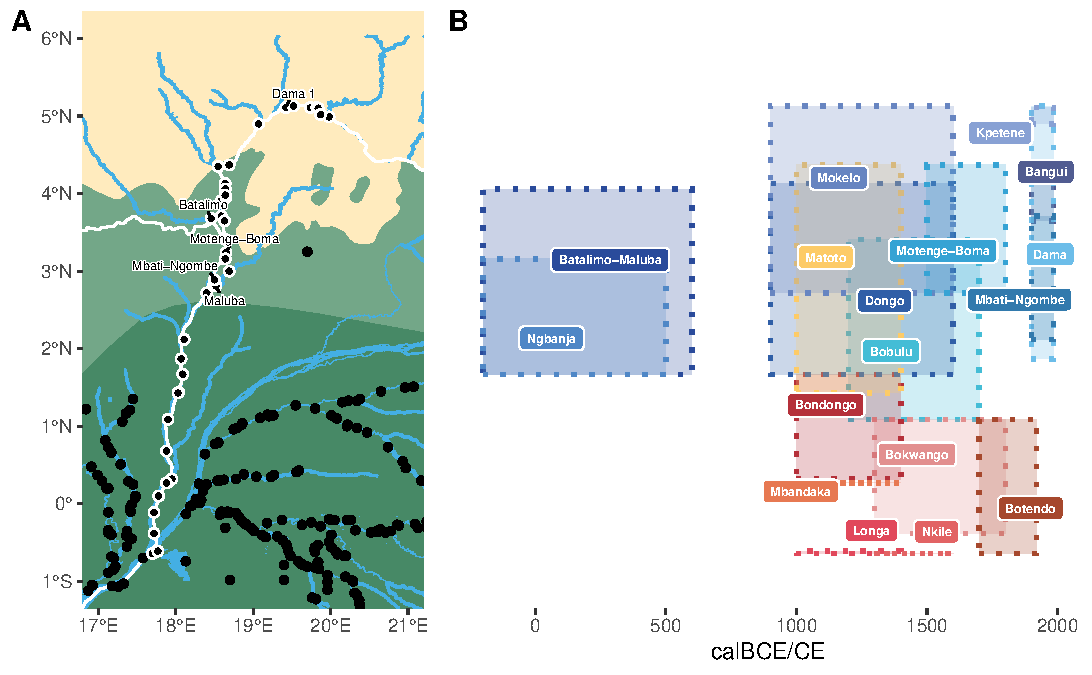
\includegraphics[width=\textwidth]{fig_ubangi_chrono.pdf}
	\caption{Map of archaeological sites along the Ubangi river (left) and chronospatial distribution of pottery styles documented within the region (right). Sites along the Ubangi show a white border, while other archaeological sites are demarcated as simple black dots. The green shading denotes the putative rainforest distribution during the 1st millennium BCE \citep{Bremond.2017,Maley.2017} (dark green) and today \citep{White.1983} (light green).}
	\label{fig:ubangi.chrono}
\end{figure*}

\subsection*{Fuzzy Border at the Ubangi river}

Another intriguing aspect concerns the importance of the surveyed river systems. Particular focus is always laid on whether rivers constitute exchange barriers or, instead, that they are preferred pathways for expansion and axes of contact \citep{Russell.2014}. The observed distribution patterns of pottery styles along the Ubangi river, a consecutive 850~km long north--south transect, show a seemingly impermeable border zone that existed for nearly two millennia \citep[Fig.~\ref{fig:ubangi.chrono};][183--185, 184 Tab.~17]{Seidensticker.2021e}. These zones are persistent and long-lasting, with ceramics rarely found outside their specific region. This 'fuzzy' boundary is situated between 1° to 1.5°~N, north of Impfondo. South of this region, all ceramics date into the Late Iron Age and are all associated with the Equator-Co style tradition of the Inner Congo Basin \citep{Wotzka.1995}. Further upriver, near the mouth of the Lua river, the Batalimo-Maluba style is among the earlier potteries in the region. All pottery groups that follow afterwards 'respect' the southern border of the Batalimo-Maluba group (Fig.~\ref{fig:ubangi.chrono}). This observation offers a unique view into a putative lack of social connectivity along one of the major rivers in Central Africa and needs more research.

\section*{Conclusions}

While pottery styles identified in the northern parts of the study area follow independent trajectories, the styles of the western parts of the Congo Basin show substantial similarities to contemporaneous styles from the Inner Congo Basin. These similarities start with the clay sourcing, resulting in very similar macroscopic ceramic fabrics. Furthermore, while vessel shapes are sometimes different, decoration techniques and motives are nearly identical. Concerning the Pikunda-Munda style, the oldest pottery widely distributed in the western Congo Basin, strong technological similarities stand in the way of several stylistic differences. So far, this style can only be loosely associated with contemporaneous ceramics of the Inner Congo Basin. Furthermore, the Pikunda-Munda style did not develop into an individual stylistic tradition, and after its end, there are no reliable links with any younger styles in the region. More critical for the settlement history of the Congo Basin is the fact that the emergence of the Pikunda-Munda group can only be dated as about 200--300 years younger than the emergence of the first pottery production further east, in the Inner Congo Basin. This fact, also considering that it is the earliest widely distributed pottery in the "Sangha River Interval" and shows legitimate stylistic differences to the ceramics from the Inner Congo Basin, refutes any hypotheses of migrations through the Congo Basin via the "Sangha River Interval" \citep{Bostoen.2015,Grollemund.2015,Grollemund.2023}.

After the setback in human activity during the 7th to 10th centuries CE, pottery groups such as the Ngombe style appear that show close stylistic ties to pottery from the Equator Co-Tradition and can be regarded as part of them. The same general association as western offshoots of the Equator Co-Tradition goes for the younger styles Ebambe and Epena.

The introduction of roulette decorations, which often govern decoration practices of modern-day ceramics, is equally vital for the region's settlement history. A gradual adoption and intensive use of this ornamentation practice can be observed within the Ngoko tradition. In the extreme south of the study area, another distinct line of pottery development was observed within the grog-tempered Bobusa group.

The settlement sequence of the northern and western Congo Basin sketched out within this study must, at least in part, be taken cautiously due to the limited sources available. Only new fieldwork and excavations can remedy this situation. Thus far, the available data constitutes valid proof for the chrono-temporal position of the early parts of the sequence during the Early Iron Age. However, available data from the middle of the 1st millennium CE onwards must be considered incomplete. Despite the extensive body of material obtained by the \textit{River Reconnaissance Project} in the 1980s, the present work only provides a first insight into the ceramic variability of the region.

\begin{acknowledgements}
Thanks go to Manfred K. H. Eggert for granting access to the finds from his project and supporting the research. Additional thanks go to Hans-Peter Wotzka for advising the research from 2012 to 2016 and Thomas Knopf as well as Manfred K. H. Eggert for their supervision afterwards. Katharina Jungnickel deserves thanks for commenting on an earlier draft of this paper. I further thank the two anonymous reviewers whose comments and suggestions greatly improved the paper.

Newly obtained radiocarbon dates on food crusts, dated at the radiocarbon dating laboratory of the Royal Institute for Cultural Heritage in Brussels (RICH) were funded by the FWO postdoctoral scholarship (1287922N) granted to the author.

All data and computer code generated during this research is available here: \url{https://github.com/dirkseidensticker/PikundaMunda_BatalimoMaluba_AAR}.
\end{acknowledgements}

\bibliographystyle{spbasic}
\bibliography{references.bib}

\end{document}
